%%% title presenaca25ss1k
\documentclass[landscape,10pt]{article}
\usepackage{pict2e}
\usepackage{ketpic2e,ketlayer2e}
\special{papersize=\the\paperwidth,\the\paperheight}
\usepackage{ketslide}
\usepackage{amsmath,amssymb}
\usepackage{bm,enumerate}
\usepackage[dvipdfmx]{graphicx}
\usepackage{color}
\usepackage[colorlinks=true,linkcolor=blue,filecolor=blue]{hyperref}
\usepackage{qrcode}
\usepackage{setspace}
\usepackage{xcolor}

\def\deg#1{#1^{\circ}}
\def\bs{$\backslash$}
\newcommand{\monthday}{0715}

\definecolor{slidecolora}{cmyk}{0.98,0.13,0,0.43}
\definecolor{slidecolorb}{cmyk}{0.2,0,0,0}
\definecolor{slidecolorc}{cmyk}{0.2,0,0,0}
\definecolor{slidecolord}{cmyk}{0.2,0,0,0}
\definecolor{slidecolore}{cmyk}{0,0,0,0.5}
\definecolor{slidecolorf}{cmyk}{0,0,0,0.5}
\definecolor{slidecolori}{cmyk}{0.98,0.13,0,0.43}
\def\setthin#1{\def\thin{#1}}
\setthin{0}
\newcounter{pagectr}
\setcounter{pagectr}{1}
\newcommand{\slidepage}[1][\monthday-]{%
\setcounter{ketpicctra}{18}%

\begin{layer}{118}{0}
\putnotew{130}{-\theketpicctra.05}{\small#1\thepage/\pageref{pageend}}
\end{layer}

}

\setmargin{20}{135}{15}{100}

\ketslideinit

\pagestyle{empty}

\begin{document}

\begin{layer}{120}{0}
\putnotese{0}{0}{{\Large\bf
\color[cmyk]{1,1,0,0}

\begin{layer}{120}{0}
{\Huge \putnotes{64}{15}{\LARGE {Development of methods for interactive classes}}}
\putnotes{62}{27}{\LARGE {using KeTLMS}}
\putnotes{62}{68}{Koji Nishiura, Setsuo Takato}
\putnotee{70}{87}{2024.12.10 ATCM2024}
\end{layer}

}
}
\end{layer}

\def\mainslidetitley{22}
\def\ketcletter{slidecolora}
\def\ketcbox{slidecolorb}
\def\ketdbox{slidecolorc}
\def\ketcframe{slidecolord}
\def\ketcshadow{slidecolore}
\def\ketdshadow{slidecolorf}
\def\slidetitlex{6}
\def\slidetitlesize{1.3}
\def\mketcletter{slidecolori}
\def\mketcbox{yellow}
\def\mketdbox{yellow}
\def\mketcframe{yellow}
\def\mslidetitlex{62}
\def\mslidetitlesize{2}

\color{black}
\Large\bf\boldmath
\addtocounter{page}{-1}

\renewcommand{\eda}[2][\theedactr]{%
\setcounter{edactr}{#1}
\Ltab{\theedawidth mm}{[#1]\ #2}%
\addtocounter{edactr}{1}%
}
\definecolor{mygreen}{rgb}{0.9,1,0.7}
\setthin{0.1}
\def\colorthin{\color[cmyk]{\thin,\thin,\thin,\thin}}
\def\dint{\displaystyle\int}
\newcommand{\dpar}[2]{\dfrac{\partial #1}{\partial #2}}
\newcommand{\dps}{\displaystyle}
\newcommand{\dpint}{\displaystyle\int}
\renewcommand{\slidepage}[1][s]{%
\setcounter{ketpicctra}{18}%
\hypersetup{linkcolor=black}%
\begin{layer}{118}{0}
\putnotee{105}{-\theketpicctra.05}{\small\monthday-\thepage/\pageref{pageend}}
\end{layer}\hypersetup{linkcolor=blue}
}
\newcommand{\setwidth}[1]{\setcounter{txtLiii}{#1}}
\newcommand{\adde}{\addtocounter{enm}{1}}
%%\newcommand{enminit}{\setcounter{enm}{1}}
\newcommand\pnp{(\theenm)}
\newcommand\pt{・}
\renewcommand{\monban}[1][\monthday]{%
#1-\themban\,%
\addtocounter{mban}{1}%
}
\renewcommand{\monbannoadd}[1][\monthday]{%
#1-\themban\,%
}
\newcommand{\eds}[1][1]{\setcounter{edactr}{#1}}%
\newcommand{\footslide}[3][]{\putnotee{5}{#2}{{\color{blue}\small *#1:#3}}}
\newcommand{\addrem}[1]{{\color{blue}{}\scriptsize\;\raisebox{3mm}{*#1}}}
\setcounter{figure}{1}
%%%%%%%%%%%%

%%%%%%%%%%%%%%%%%%%%

\mainslide{Outline of Today's Talk}


\slidepage[m]
%%%%%%%%%%%%

%%%%%%%%%%%%%%%%%%%%

\newslide{What is Algebrite}

\vspace*{18mm}

\slidepage
\enminit
\textinit[104]

\begin{layer}{120}{0}
\addtext{8}{\ten}{Algebrite is a library for CAS. It can run in the html.}
\addtext[10]{8}{\ten}{Prof. Kitamoto made a command `\mbox{\tt\color{red}exealg}', which allows Algebrite and KeTCindyJS to collaborate.}
\addtext[14]{8}{\ten}{We use `{\tt\color{red}exealg}' in KeTTask (which is based on KeTCindyJS).}
\end{layer}

%%%%%%%%%%%%

%%%%%%%%%%%%%%%%%%%%


\newslide{What is KeTLTS}

\vspace*{18mm}

\slidepage
\enminit
\textinit

\begin{layer}{120}{0}
\addtext{8}{2020}{Covid-19 changed classes drastically.}
\addtext{8}{\ten}{Online classes became mainstream in many schools.}
\addtext[8]{8}{\ten}{Mathematics classes were no exception.}
\addtext{8}{\ten}{Teachers faced the big issue of how to exchange mathematical formulas. }
\end{layer}

%%%%%%%%%%%%

%%%%%%%%%%%%%%%%%%%%


\sameslide

\vspace*{18mm}

\slidepage
\enminit
\textinit

\begin{layer}{120}{0}
\addtext{8}{2020}{Covid-19 changed classes drastically.}
\addtext{8}{\ten}{Online classes became mainstream in many schools.}
\addtext[8]{8}{\ten}{Mathematics classes were no exception.}
\addtext{8}{\ten}{Teachers faced the big issue of how to exchange mathematical formulas. }
\putnotew{50}{60}{\fbox{Teacher}}\putnotee{66}{60}{\fbox{Student}}
\end{layer}


\sameslide

\vspace*{18mm}

\slidepage
\enminit
\textinit

\begin{layer}{120}{0}
\addtext{8}{2020}{Covid-19 changed classes drastically.}
\addtext{8}{\ten}{Online classes became mainstream in many schools.}
\addtext[8]{8}{\ten}{Mathematics classes were no exception.}
\addtext{8}{\ten}{Teachers faced the big issue of how to exchange mathematical formulas. }
\putnotew{50}{60}{\fbox{Teacher}}\putnotee{66}{60}{\fbox{Student}}
\putnotec{58}{56}{$\xrightarrow{easy}$}
\end{layer}


\sameslide

\vspace*{18mm}

\slidepage
\enminit
\textinit

\begin{layer}{120}{0}
\addtext{8}{2020}{Covid-19 changed classes drastically.}
\addtext{8}{\ten}{Online classes became mainstream in many schools.}
\addtext[8]{8}{\ten}{Mathematics classes were no exception.}
\addtext{8}{\ten}{Teachers faced the big issue of how to exchange mathematical formulas. }
\putnotew{50}{60}{\fbox{Teacher}}\putnotee{66}{60}{\fbox{Student}}
\putnotec{58}{56}{$\xrightarrow{easy}$}
\putnotec{58}{64}{$\xleftarrow[hard]{}$}
\end{layer}


\sameslide

\vspace*{18mm}

\slidepage
\enminit
\textinit

\begin{layer}{120}{0}
\addtext{8}{2020}{Covid-19 changed classes drastically.}
\addtext{8}{\ten}{Online classes became mainstream in many schools.}
\addtext[8]{8}{\ten}{Mathematics classes were no exception.}
\addtext{8}{\ten}{Teachers faced the big issue of how to exchange mathematical formulas. }
\putnotew{50}{60}{\fbox{Teacher}}\putnotee{66}{60}{\fbox{Student}}
\putnotec{58}{56}{$\xrightarrow{easy}$}
\putnotec{58}{64}{$\xleftarrow[hard]{}$}
\addtext[20]{8}{\ten}{We decided to develop KeTLTS.}
\end{layer}


\sameslide

\vspace*{18mm}

\slidepage
\enminit
\textinit

\begin{layer}{120}{0}
\addtext{8}{2020}{Covid-19 changed classes drastically.}
\addtext{8}{\ten}{Online classes became mainstream in many schools.}
\addtext[8]{8}{\ten}{Mathematics classes were no exception.}
\addtext{8}{\ten}{Teachers faced the big issue of how to exchange mathematical formulas. }
\putnotew{50}{60}{\fbox{Teacher}}\putnotee{66}{60}{\fbox{Student}}
\putnotec{58}{56}{$\xrightarrow{easy}$}
\putnotec{58}{64}{$\xleftarrow[hard]{}$}
\addtext[20]{8}{\ten}{We decided to develop KeTLTS.}
\putnotee{15}{4}{\color{blue}KeTCindy Learning data Transfer System}
\end{layer}


\newslide{Developing KeTMath}

\vspace*{18mm}

\slidepage
\enminit
\textinit

\begin{layer}{120}{0}
\addtext{8}{\ten}{This system uses only one line text.}
\addtext{20}{*}{It is lightweight and easy to process.}
%%\settext{8}{8}{115}
%%\settext{8}{8}{110}
\end{layer}

%%%%%%%%%%%%

%%%%%%%%%%%%%%%%%%%%


\sameslide

\vspace*{18mm}

\slidepage
\enminit
\textinit

\begin{layer}{120}{0}
\addtext{8}{\ten}{This system uses only one line text.}
\addtext{20}{*}{It is lightweight and easy to process.}
\addtext{8}{\ten}{The followings are required}
\addtext{18}{(1)}{Conversion Rules (KeTMath Rules)}
\end{layer}


\sameslide

\vspace*{18mm}

\slidepage
\enminit
\textinit

\begin{layer}{120}{0}
\addtext{8}{\ten}{This system uses only one line text.}
\addtext{20}{*}{It is lightweight and easy to process.}
\addtext{8}{\ten}{The followings are required}
\addtext{18}{(1)}{Conversion Rules (KeTMath Rules)}
\addtext{18}{(2)}{Function to convert a text to \TeX\ format}
\addtext{20}{*}{CindyJS implements KaTeX (v0.8).}
\addtext{26}{}{It displays expressions as 2D in HTML.}
\end{layer}


\newslide{KeTMath}

\vspace*{18mm}

\slidepage
\enminit
\textinit

\begin{layer}{120}{0}
\addtext{8}{\ten}{KeTMath Rules}
\addtext{16}{}{Here are some typical examples.}
\addtext{24}{}{fr(a,b) $\Longrightarrow$ $\dfrac{a}{b}$}
\addtext[2]{24}{}{sq(n,a) $\Longrightarrow$ $\sqrt[n]{a}$}
\addtext{24}{}{diff(y,x) $\Longrightarrow$ $\frac{dy}{dx}$}
\end{layer}

%%%%%%%%%%%%
%%new::Screen of ketmath.html
%%%repeat=7
%%\slidepage
%%%%%%%%%%%%

%%%%%%%%%%%%%%%%%%%%


\sameslide

\vspace*{18mm}

\slidepage
\enminit
\textinit

\begin{layer}{120}{0}
\addtext{8}{\ten}{KeTMath Rules}
\addtext{16}{}{Here are some typical examples.}
\addtext{24}{}{fr(a,b) $\Longrightarrow$ $\dfrac{a}{b}$}
\addtext[2]{24}{}{sq(n,a) $\Longrightarrow$ $\sqrt[n]{a}$}
\addtext{24}{}{diff(y,x) $\Longrightarrow$ $\frac{dy}{dx}$}
\addtext{8}{\ten}{Conversion Functions}
\addtext{24}{}{Totexform,Tocindyform,Tomaxform}
\end{layer}


\newslide{Development of KeTLTS}

\vspace*{18mm}

\slidepage
\textinit[110]

\begin{layer}{120}{0}
\addtext{8}{\ten}{`kettask(+ID).html' is created by adding question data to
the template file.}
\end{layer}

%%%%%%%%%%%%

%%%%%%%%%%%%%%%%%%%%


\sameslide

\vspace*{18mm}

\slidepage
\textinit[110]

\begin{layer}{120}{0}
\addtext{8}{\ten}{`kettask(+ID).html' is created by adding question data to
the template file.}
\addtext[8]{8}{\ten}{It exchanges questions and answers
 written in KeTMath rules.}
\end{layer}


\sameslide

\vspace*{18mm}

\slidepage
\textinit[110]

\begin{layer}{120}{0}
\addtext{8}{\ten}{`kettask(+ID).html' is created by adding question data to
the template file.}
\addtext[8]{8}{\ten}{It exchanges questions and answers
 written in KeTMath rules.}
\addtext[8]{8}{\ten}{`toolketmath.cdy' creates the html file.}
\end{layer}


\newslide{Initial screen of kettask}

\vspace*{18mm}

\slidepage
\enminit
\textinit[115]

\begin{layer}{120}{0}
\putnotes{65}{0}{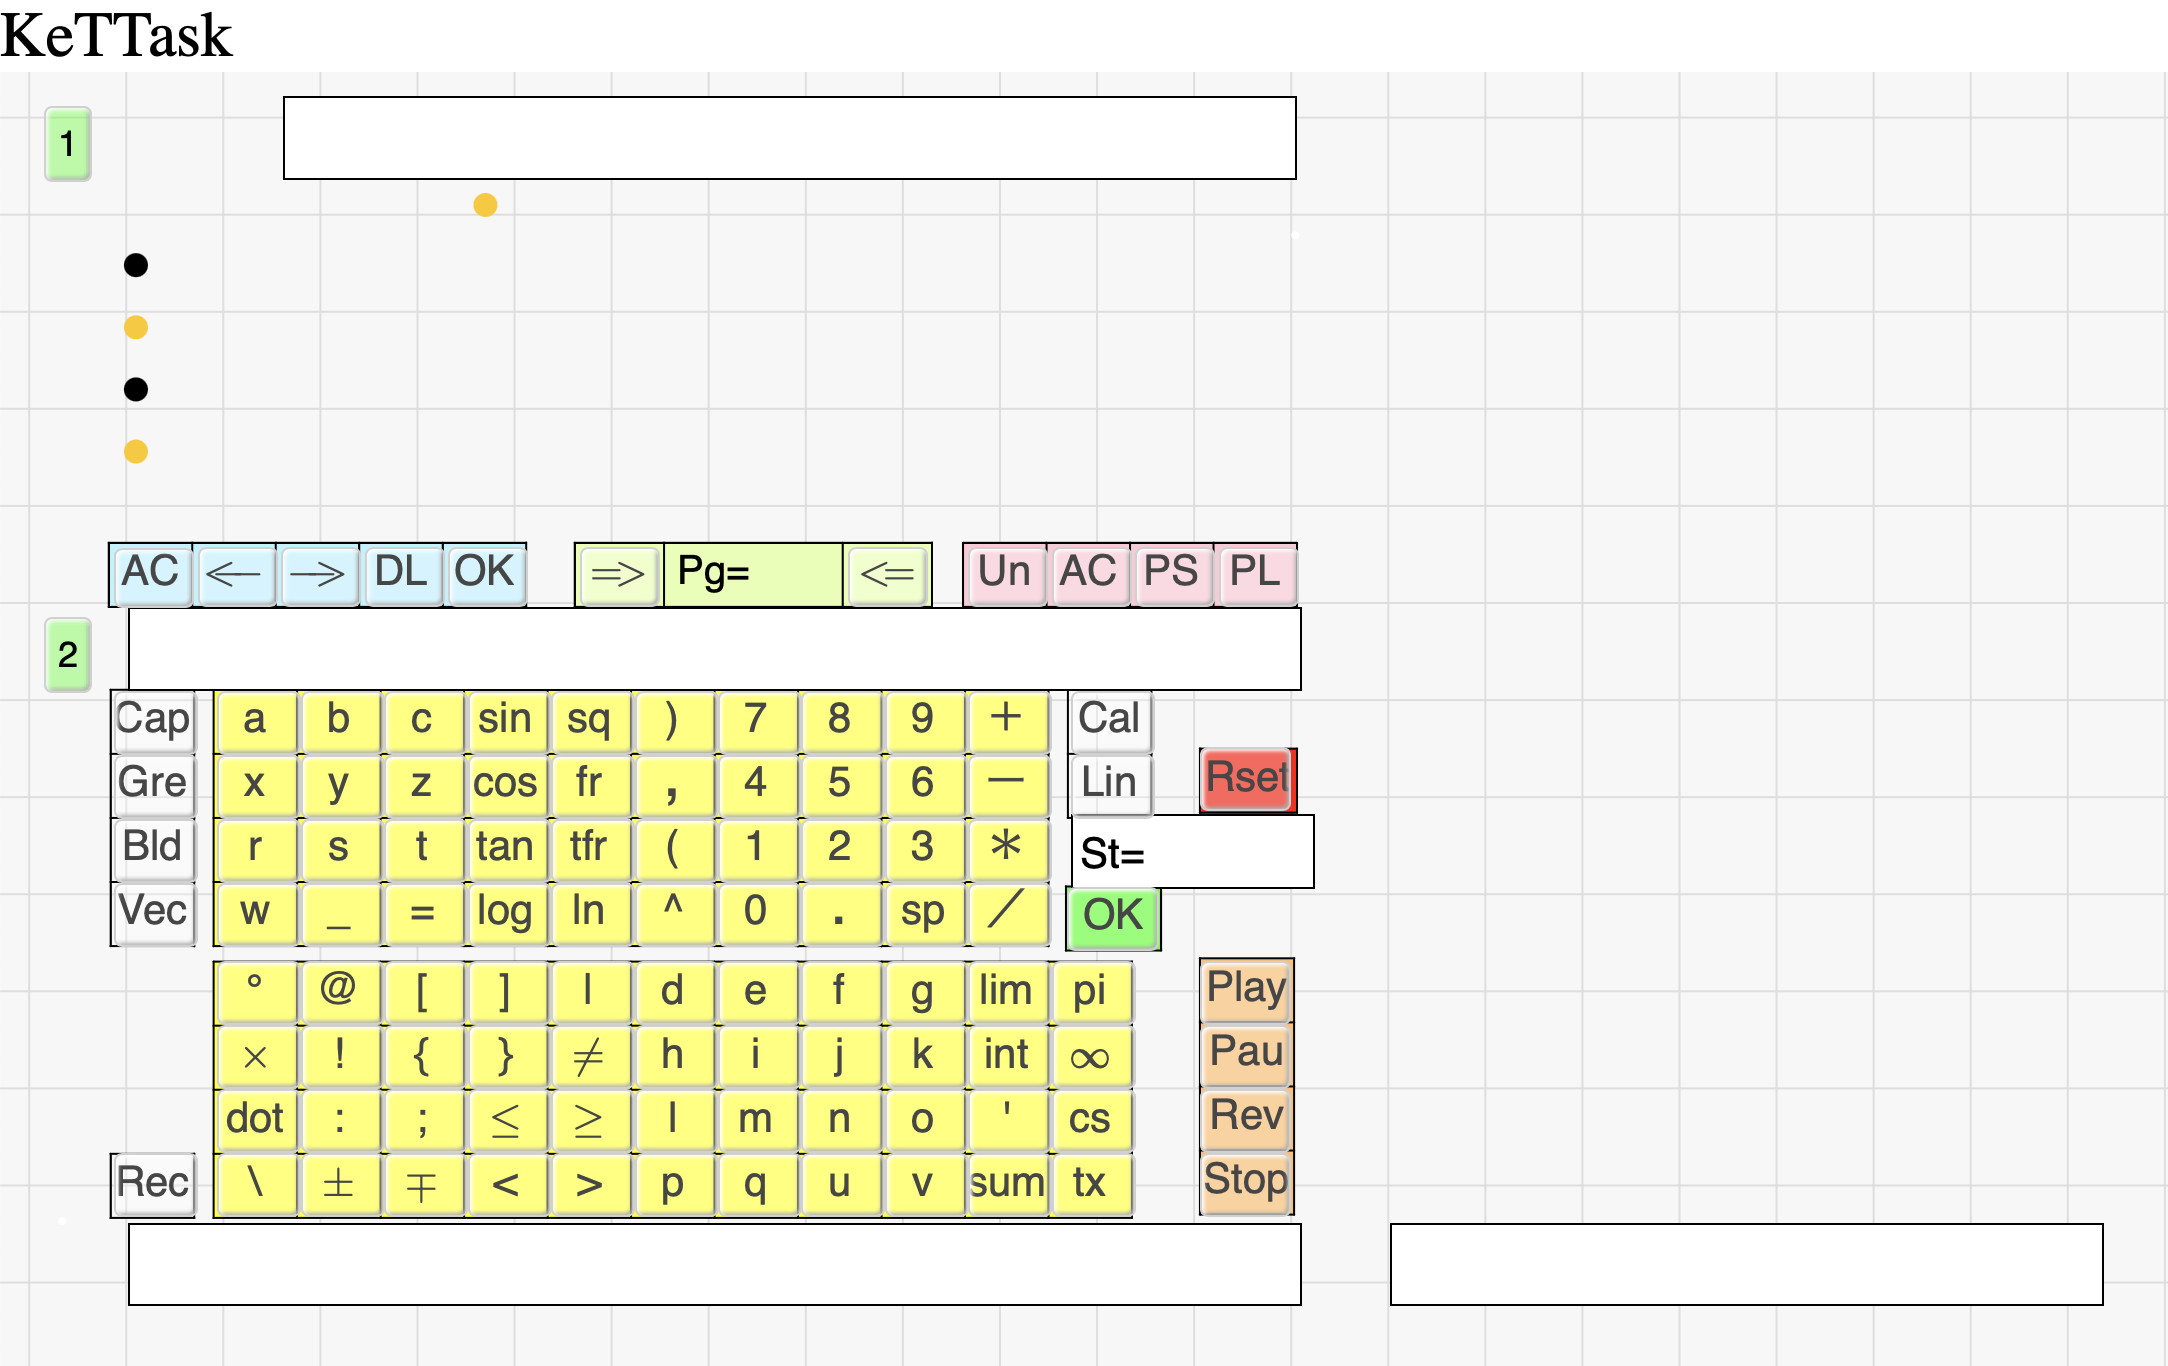
\includegraphics[width=100mm]{fig/kettaskinit.png}
}
\end{layer}

%%%%%%%%%%%%

%%%%%%%%%%%%%%%%%%%%


\newslide{How to create kettask.html}

\vspace*{18mm}

\slidepage
\enminit
\textinit[115]

\begin{layer}{120}{0}
\addtext[-4]{8}{\pnp}{Goto `ketcindy home'.}\adde
\addtext{16}{}{\normalsize \url{https://s-takato.github.io/ketcindyorg/indexe.html}}
\addtext{8}{\pnp}{Install Cinderella.}\adde
\addtext{8}{\pnp}{Download KeTLTS.}\adde
\addtext{16}{}{I use the bare minimum\\ of files in `work'.}
\addtext[8]{8}{\pnp}{I will explain the rest\\by actually running it.}
\putnotese{83}{22}{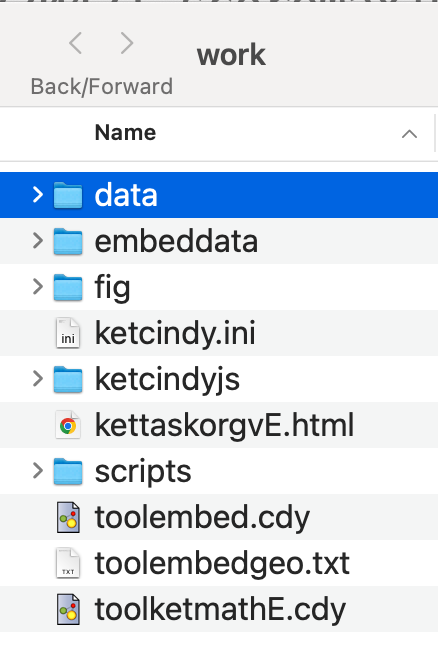
\includegraphics[width=35mm]{fig/kettaskwork.png}}
\end{layer}

%%%%%%%%%%%%

%%%%%%%%%%%%%%%%%%%%


\newslide{How to create questions}

\vspace*{18mm}

\slidepage
\enminit
\textinit[110]
{%%\normalsize

\begin{layer}{120}{0}
\addtext[-4]{8}{\ten}{Go to `work/data'}
\addtext{8}{\ten}{Open 'student2025.txt' and register students.}
\addtext[6]{8}{\ten}{Open 'question(001-1).txt' and write questions.}
\putnotes{65}{33}{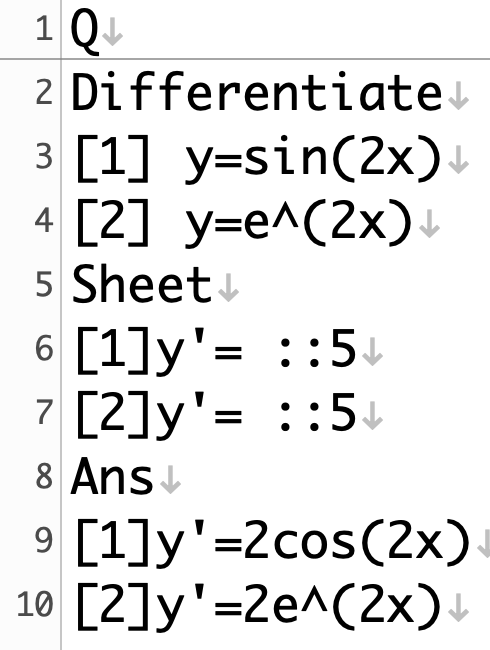
\includegraphics[width=25mm]{fig/questions.png}}
\end{layer}

}
%%%%%%%%%%%%

%%%%%%%%%%%%%%%%%%%%


\newslide{How to create kettask(xxx).html}

\vspace*{18mm}

\slidepage
\enminit
\textinit[110]

\begin{layer}{120}{0}
\addtext[-4]{8}{\ten}{\normalsize Launch `toolketmathE.cdy'}
\textinit[45]
\addtext[4]{8}{\ten}{\normalsize Click `1.taskline' and 'Go'}
\putnotesw{125}{10}{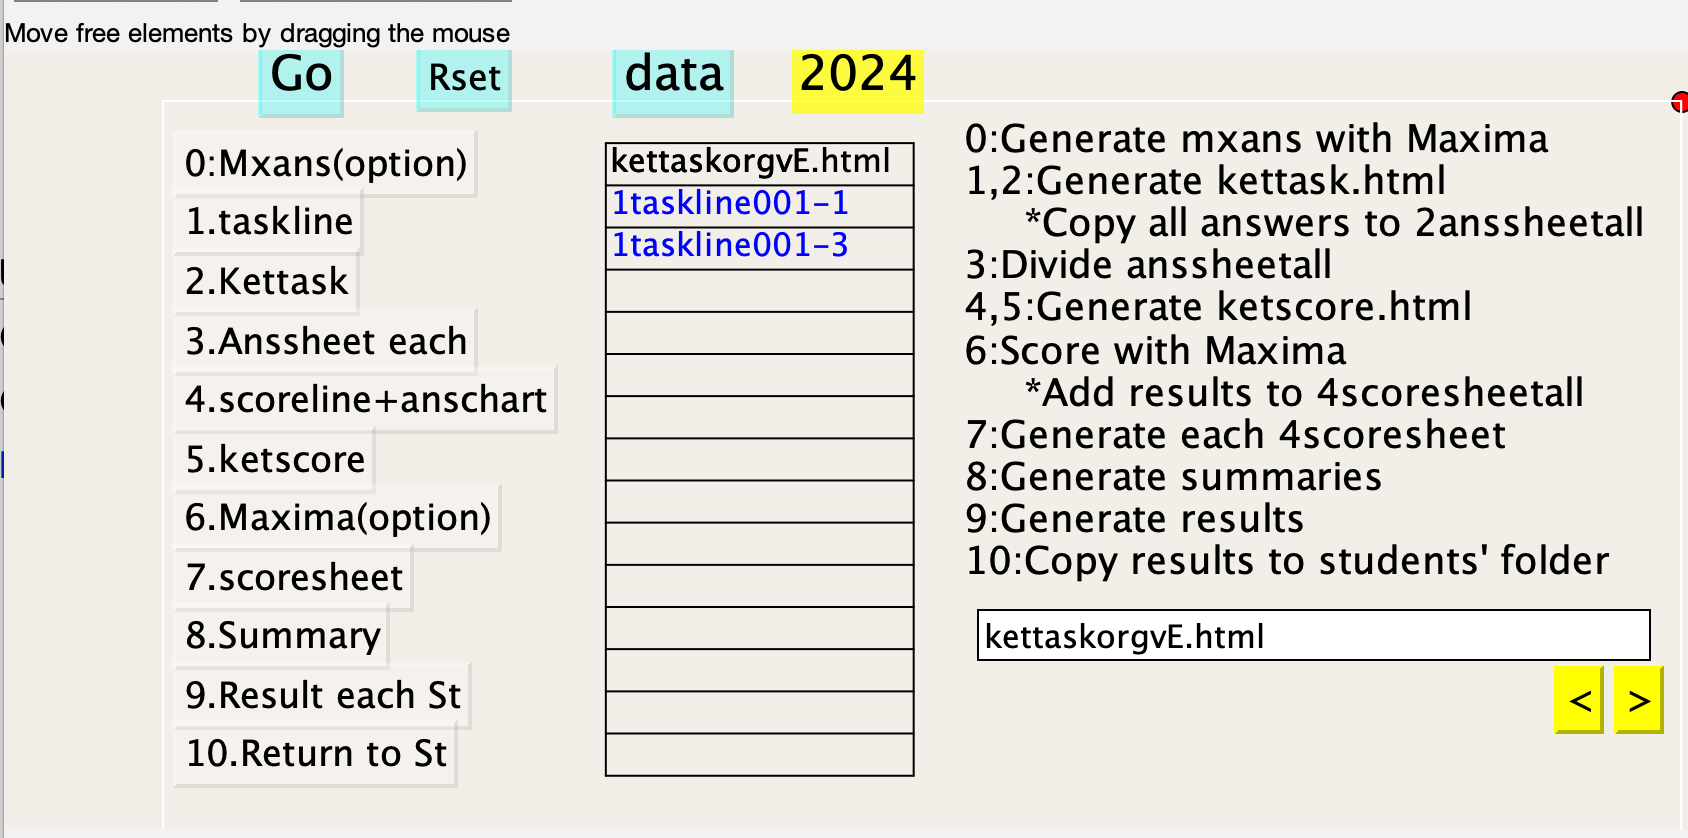
\includegraphics[width=60mm]{fig/toolketmath1.png}}
\end{layer}

%%%%%%%%%%%%
%%new::Screen of kettask.html
%%%repeat=2
%%\slidepage
%%
%%\enminit
%%\textinit
%%
%%\vspace{2mm}
%%...
%%{\normalsize
%%layer::{120}{0}
%%%[1]::\putnotese{3}{2}{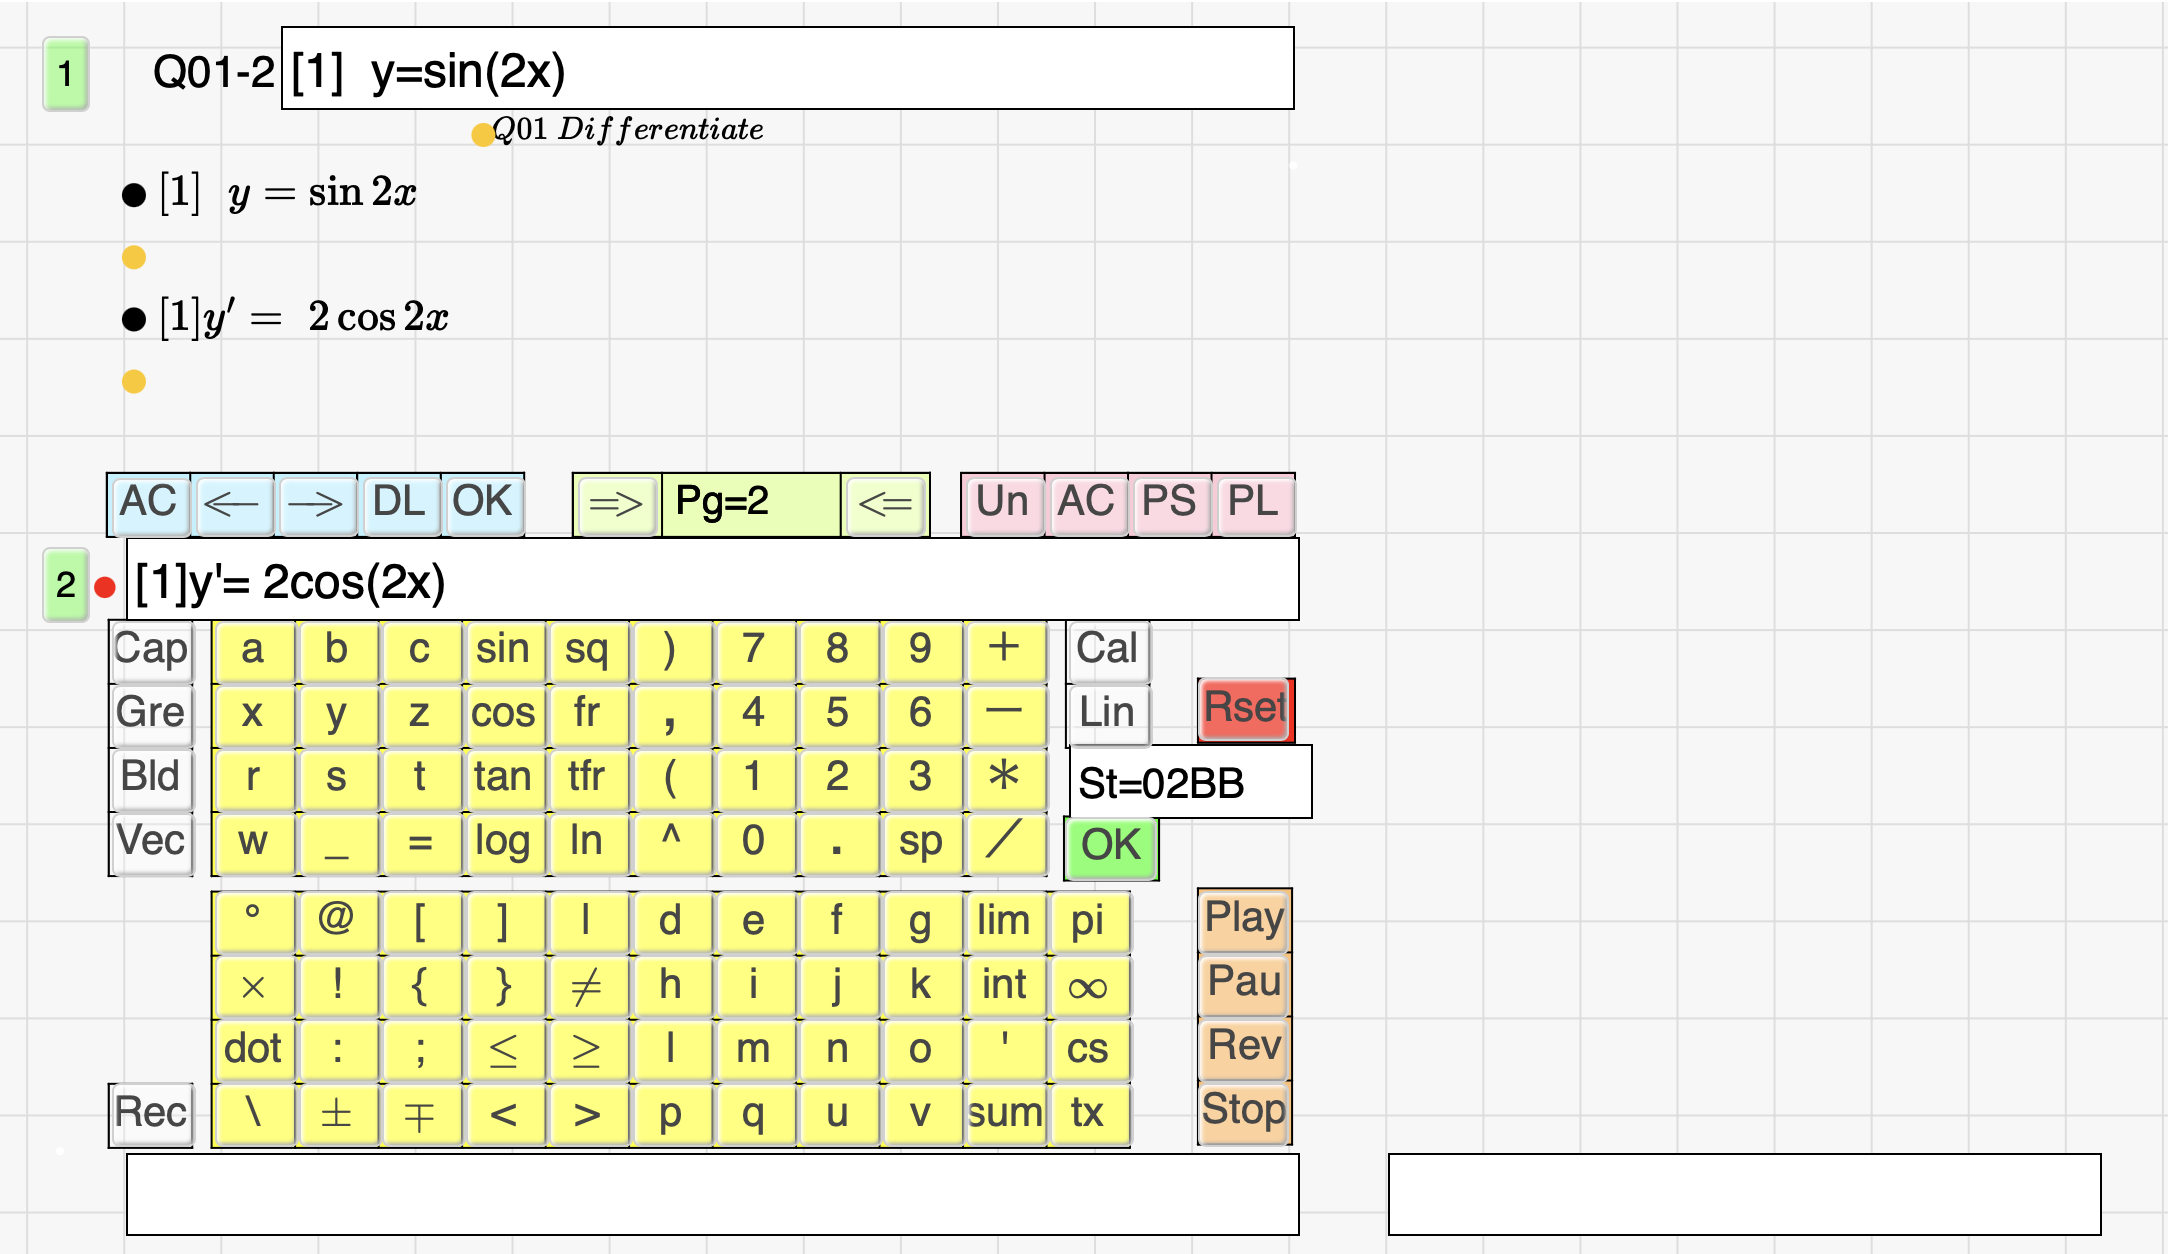
\includegraphics[width=120mm]{fig/kettask10.png}}
%%%[2]::\putnotese{3}{2}{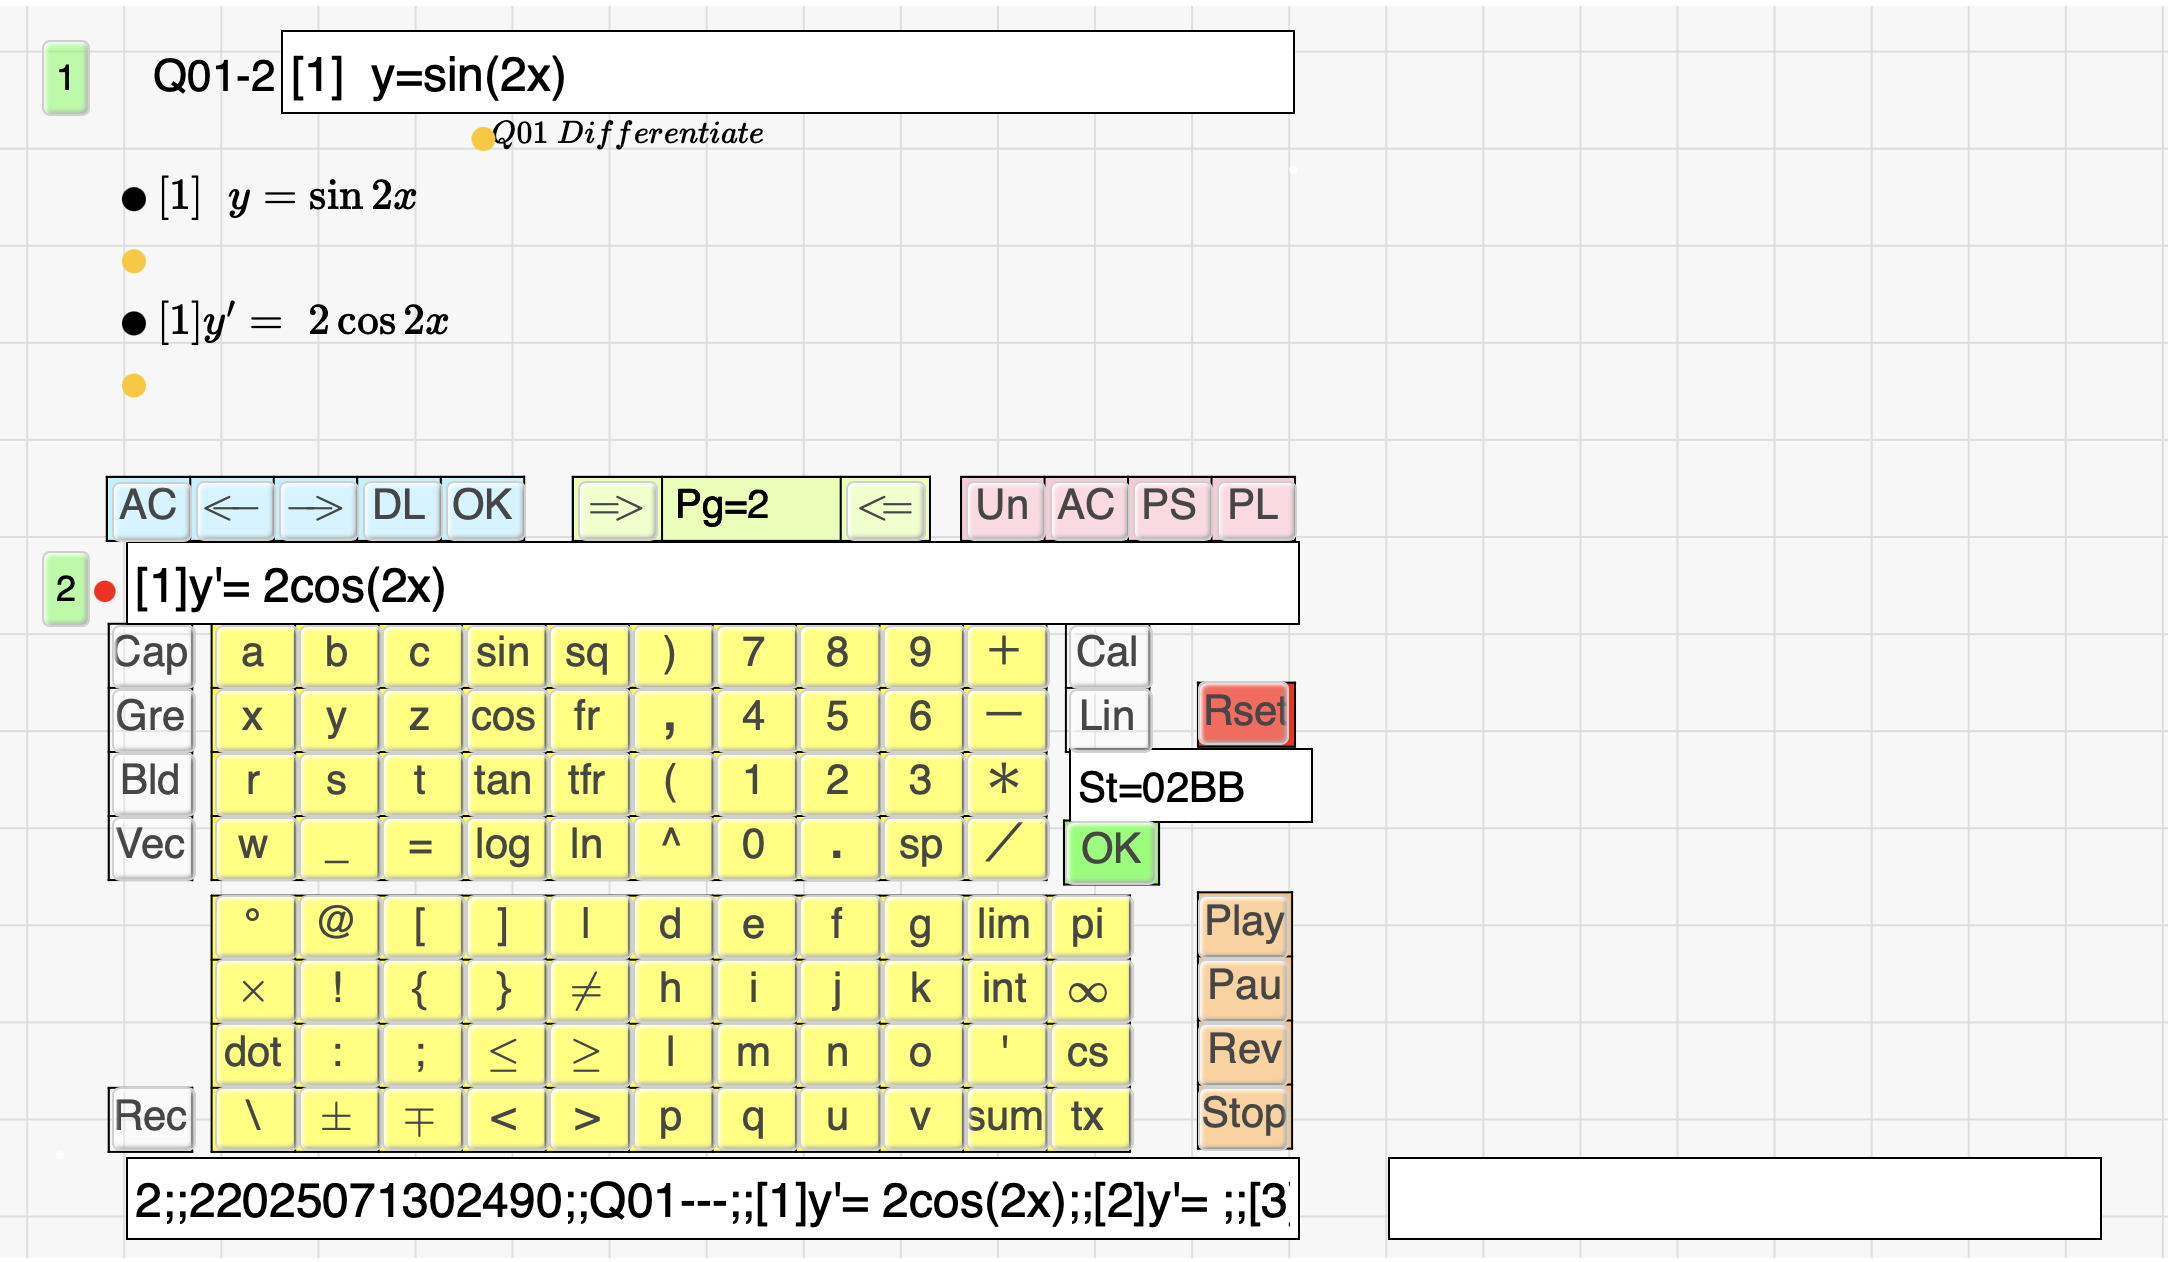
\includegraphics[width=120mm]{fig/kettask11.png}}
%%\addtext[-8]{78}{\pnp}{Initial Screen}\adde
%%\addtext[-4]{78}{\pnp}{St=num, Click \scalebox{.9}{\fcolorbox{black}{green}{\tt OK}}}\adde
%%\addtext[-2]{78}{\pnp}{Confirm StudentID}\adde
%%\addtext[-4]{78}{\pnp}{Click \scalebox{.9}{\fcolorbox{black}{green}{\tt OK}} again}\adde
%%\addtext[-3]{78}{\pnp}{Click \scalebox{.9}{\fcolorbox{black}{mygreen}{\tt $=\!>\!$}}}\adde
%%\addtext[-3]{78}{\pnp}{Input \fcolorbox{black}{yellow}{\tt 2}}\adde
%%\addtext[-3]{78}{\pnp}{Click \fcolorbox{black}{yellow}{\tt cos}}\adde
%%\addtext[-3]{78}{\pnp}{Input 2x}\adde
%%\addtext[-4]{78}{\pnp}{Click \scalebox{.9}{\fcolorbox{black}{cyan!20}{\tt$-\!\!\!>\!$}}('?' moves)}\adde
%%\addtext[-3]{78}{\pnp}{Click \scalebox{.9}{\fcolorbox{black}{cyan!20}{\tt OK}}}\adde
%%\addtext[-3]{82}{}{'?' disappears}
%%%[2,-]::\addtext[-4]{78}{\pnp}{Click \scalebox{.85}{\fbox{\tt Rec}}}\adde
%%end
%%}
%%%%%%%%%%%%

%%%%%%%%%%%%%%%%%%%%


\sameslide

\vspace*{18mm}

\slidepage
\enminit
\textinit[110]

\begin{layer}{120}{0}
\addtext[-4]{8}{\ten}{\normalsize Launch `toolketmathE.cdy'}
\textinit[45]
\addtext[4]{8}{\ten}{\normalsize Click `1.taskline' and 'Go'}
\putnotesw{125}{10}{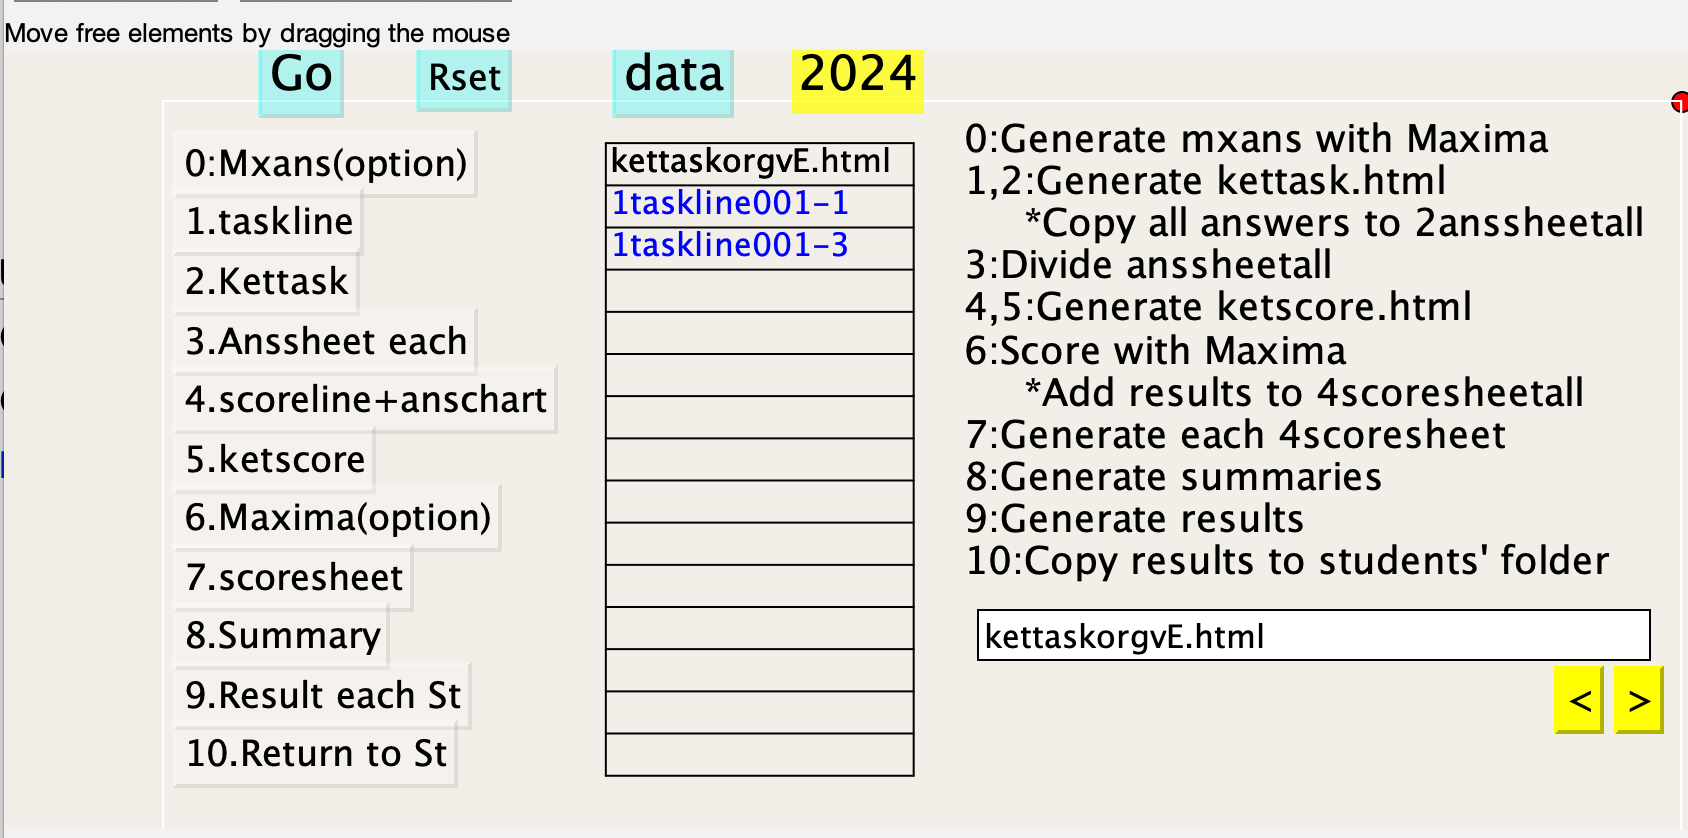
\includegraphics[width=60mm]{fig/toolketmath1.png}}
\addtext[24]{8}{\ten}{\normalsize Click `2.Ketask', select top file and `Go'}
\putnotesw{125}{44}{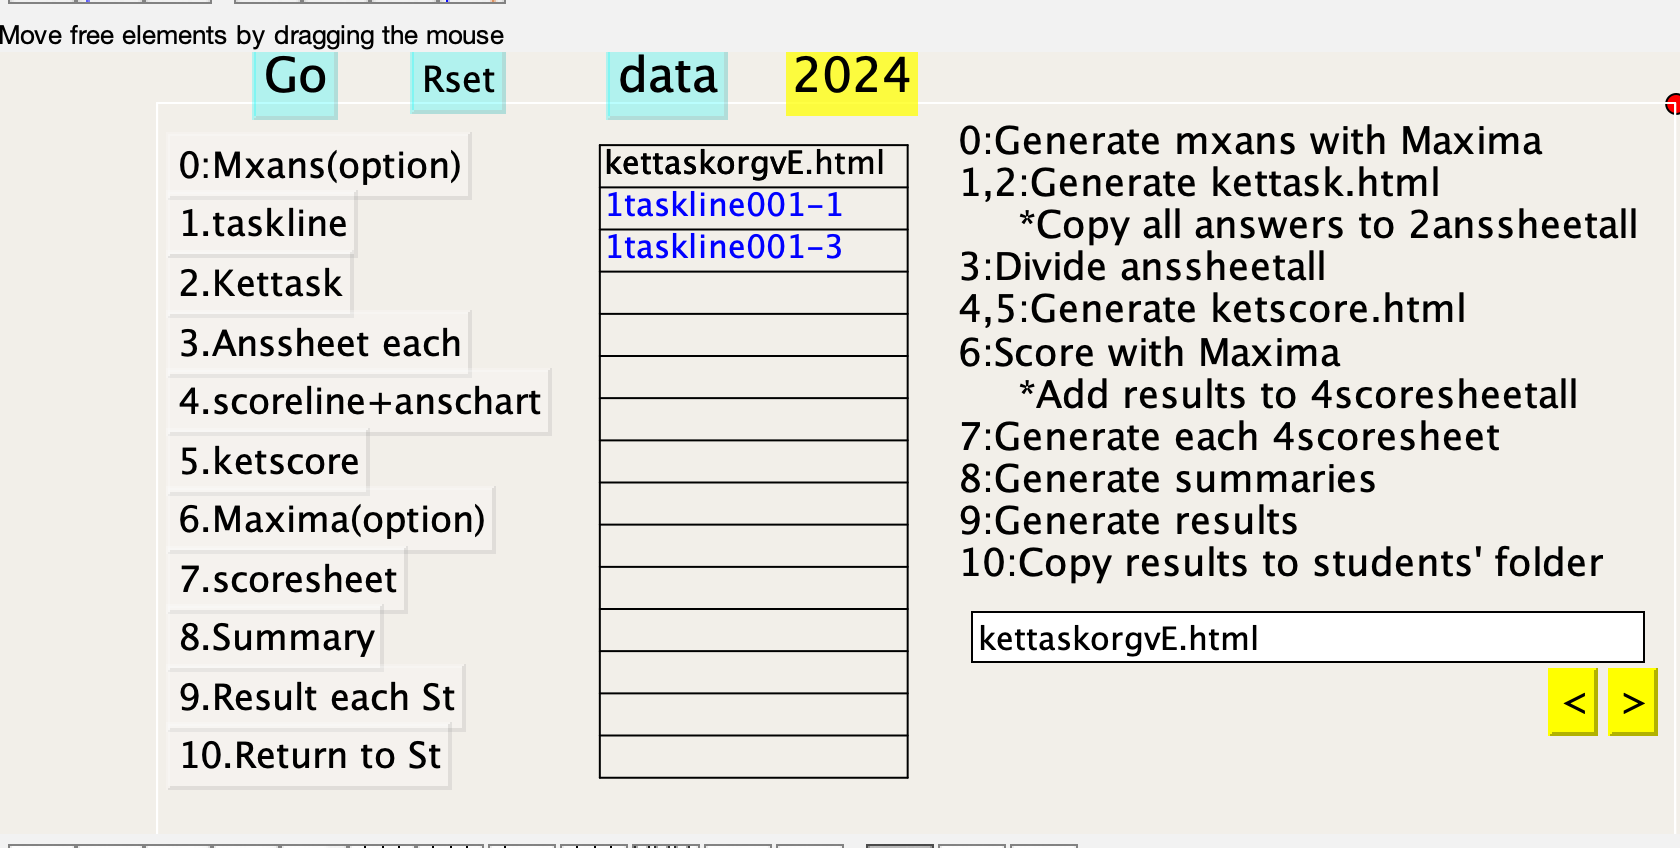
\includegraphics[width=60mm]{fig/toolketmath2.png}}
\end{layer}


\newslide{Distributing Questions}

\vspace*{18mm}

\slidepage
\enminit
\textinit[110]

\begin{layer}{120}{0}
{\normalsize
\addtext[-4]{20}{}{\color{red}The tasks for teachers creating assignments are as follows.}
}
\addtext[-2]{8}{\ten}{We upload `kettask.html' to Github Pages.}
\end{layer}

%%%%%%%%%%%%
%%new::GC Question Screen
%%%repeat=1
%%\slidepage
%%%%%%%%%%%%
%%new::GC Viewing
%%%repeat=2
%%\slidepage
%%%%%%%%%%%%

%%%%%%%%%%%%%%%%%%%%


\sameslide

\vspace*{18mm}

\slidepage
\enminit
\textinit[110]

\begin{layer}{120}{0}
{\normalsize
\addtext[-4]{20}{}{\color{red}The tasks for teachers creating assignments are as follows.}
}
\addtext[-2]{8}{\ten}{We upload `kettask.html' to Github Pages.}
\addtext{8}{\ten}{We distribute the URL to students by GC or other LMS.}
\end{layer}


\sameslide

\vspace*{18mm}

\slidepage
\enminit
\textinit[110]

\begin{layer}{120}{0}
{\normalsize
\addtext[-4]{20}{}{\color{red}The tasks for teachers creating assignments are as follows.}
}
\addtext[-2]{8}{\ten}{We upload `kettask.html' to Github Pages.}
\addtext{8}{\ten}{We distribute the URL to students by GC or other LMS.}
\addtext[6]{8}{\ten}{The data is a single line of text.}
\end{layer}


\sameslide

\vspace*{18mm}

\slidepage
\enminit
\textinit[110]

\begin{layer}{120}{0}
{\normalsize
\addtext[-4]{20}{}{\color{red}The tasks for teachers creating assignments are as follows.}
}
\addtext[-2]{8}{\ten}{We upload `kettask.html' to Github Pages.}
\addtext{8}{\ten}{We distribute the URL to students by GC or other LMS.}
\addtext[6]{8}{\ten}{The data is a single line of text.}
\addtext{8}{\ten}{The size of the data to be uploaded is small.}
\end{layer}


\sameslide

\vspace*{18mm}

\slidepage
\enminit
\textinit[110]

\begin{layer}{120}{0}
{\normalsize
\addtext[-4]{20}{}{\color{red}The tasks for teachers creating assignments are as follows.}
}
\addtext[-2]{8}{\ten}{We upload `kettask.html' to Github Pages.}
\addtext{8}{\ten}{We distribute the URL to students by GC or other LMS.}
\addtext[6]{8}{\ten}{The data is a single line of text.}
\addtext{8}{\ten}{The size of the data to be uploaded is small.}
\addtext{8}{\ten}{Teachers can send it at the appropriate time during the class.}
\end{layer}


\sameslide

\vspace*{18mm}

\slidepage
\enminit
\textinit[110]

\begin{layer}{120}{0}
{\normalsize
\addtext[-4]{20}{}{\color{red}The tasks for teachers creating assignments are as follows.}
}
\addtext[-2]{8}{\ten}{We upload `kettask.html' to Github Pages.}
\addtext{8}{\ten}{We distribute the URL to students by GC or other LMS.}
\addtext[6]{8}{\ten}{The data is a single line of text.}
\addtext{8}{\ten}{The size of the data to be uploaded is small.}
\addtext{8}{\ten}{Teachers can send it at the appropriate time during the class.}
\addtext[6]{8}{\ten}{Most students use smartphones and they can immediately receive and start answering questions.}
\end{layer}


\newslide{Collecting Data}

\vspace*{18mm}

\slidepage
\enminit
\textinit[105]

\begin{layer}{120}{0}
{\normalsize
\addtext[-4]{20}{}{\color{red}The tasks for teachers creating assignments are as follows.}
}
\addtext[-2]{8}{\ten}{Answers are collected by simply copying them onto a pre-prepared answer sheet\\ `anssheetall.txt' in the folder `data'. }
\end{layer}

%%%%%%%%%%%%

%%%%%%%%%%%%%%%%%%%%


\sameslide

\vspace*{18mm}

\slidepage
\enminit
\textinit[105]

\begin{layer}{120}{0}
{\normalsize
\addtext[-4]{20}{}{\color{red}The tasks for teachers creating assignments are as follows.}
}
\addtext[-2]{8}{\ten}{Answers are collected by simply copying them onto a pre-prepared answer sheet\\ `anssheetall.txt' in the folder `data'. }
\addtext[16]{8}{\ten}{The result `anschart.csv' can be easily generated using `toolketmath.cdy'.}
\end{layer}


\sameslide

\vspace*{18mm}

\slidepage
\enminit
\textinit[105]

\begin{layer}{120}{0}
{\normalsize
\addtext[-4]{20}{}{\color{red}The tasks for teachers creating assignments are as follows.}
}
\addtext[-2]{8}{\ten}{Answers are collected by simply copying them onto a pre-prepared answer sheet\\ `anssheetall.txt' in the folder `data'. }
\addtext[16]{8}{\ten}{The result `anschart.csv' can be easily generated using `toolketmath.cdy'.}
\addtext[8]{8}{\ten}{The point is that `anschart.csv' is a text file.}
\addtext[4]{16}{}{It can be easily processed in various ways.}
\end{layer}


\mainslide{Bundle of Algebrite}


\slidepage[m]
%%%%%%%%%%%%

%%%%%%%%%%%%%%%%%%%%

\newslide{Initial screen of kettask{\small(algbrite version)}}

\vspace*{18mm}

\slidepage
\enminit
\textinit[115]

\begin{layer}{120}{0}
\putnotes{65}{4}{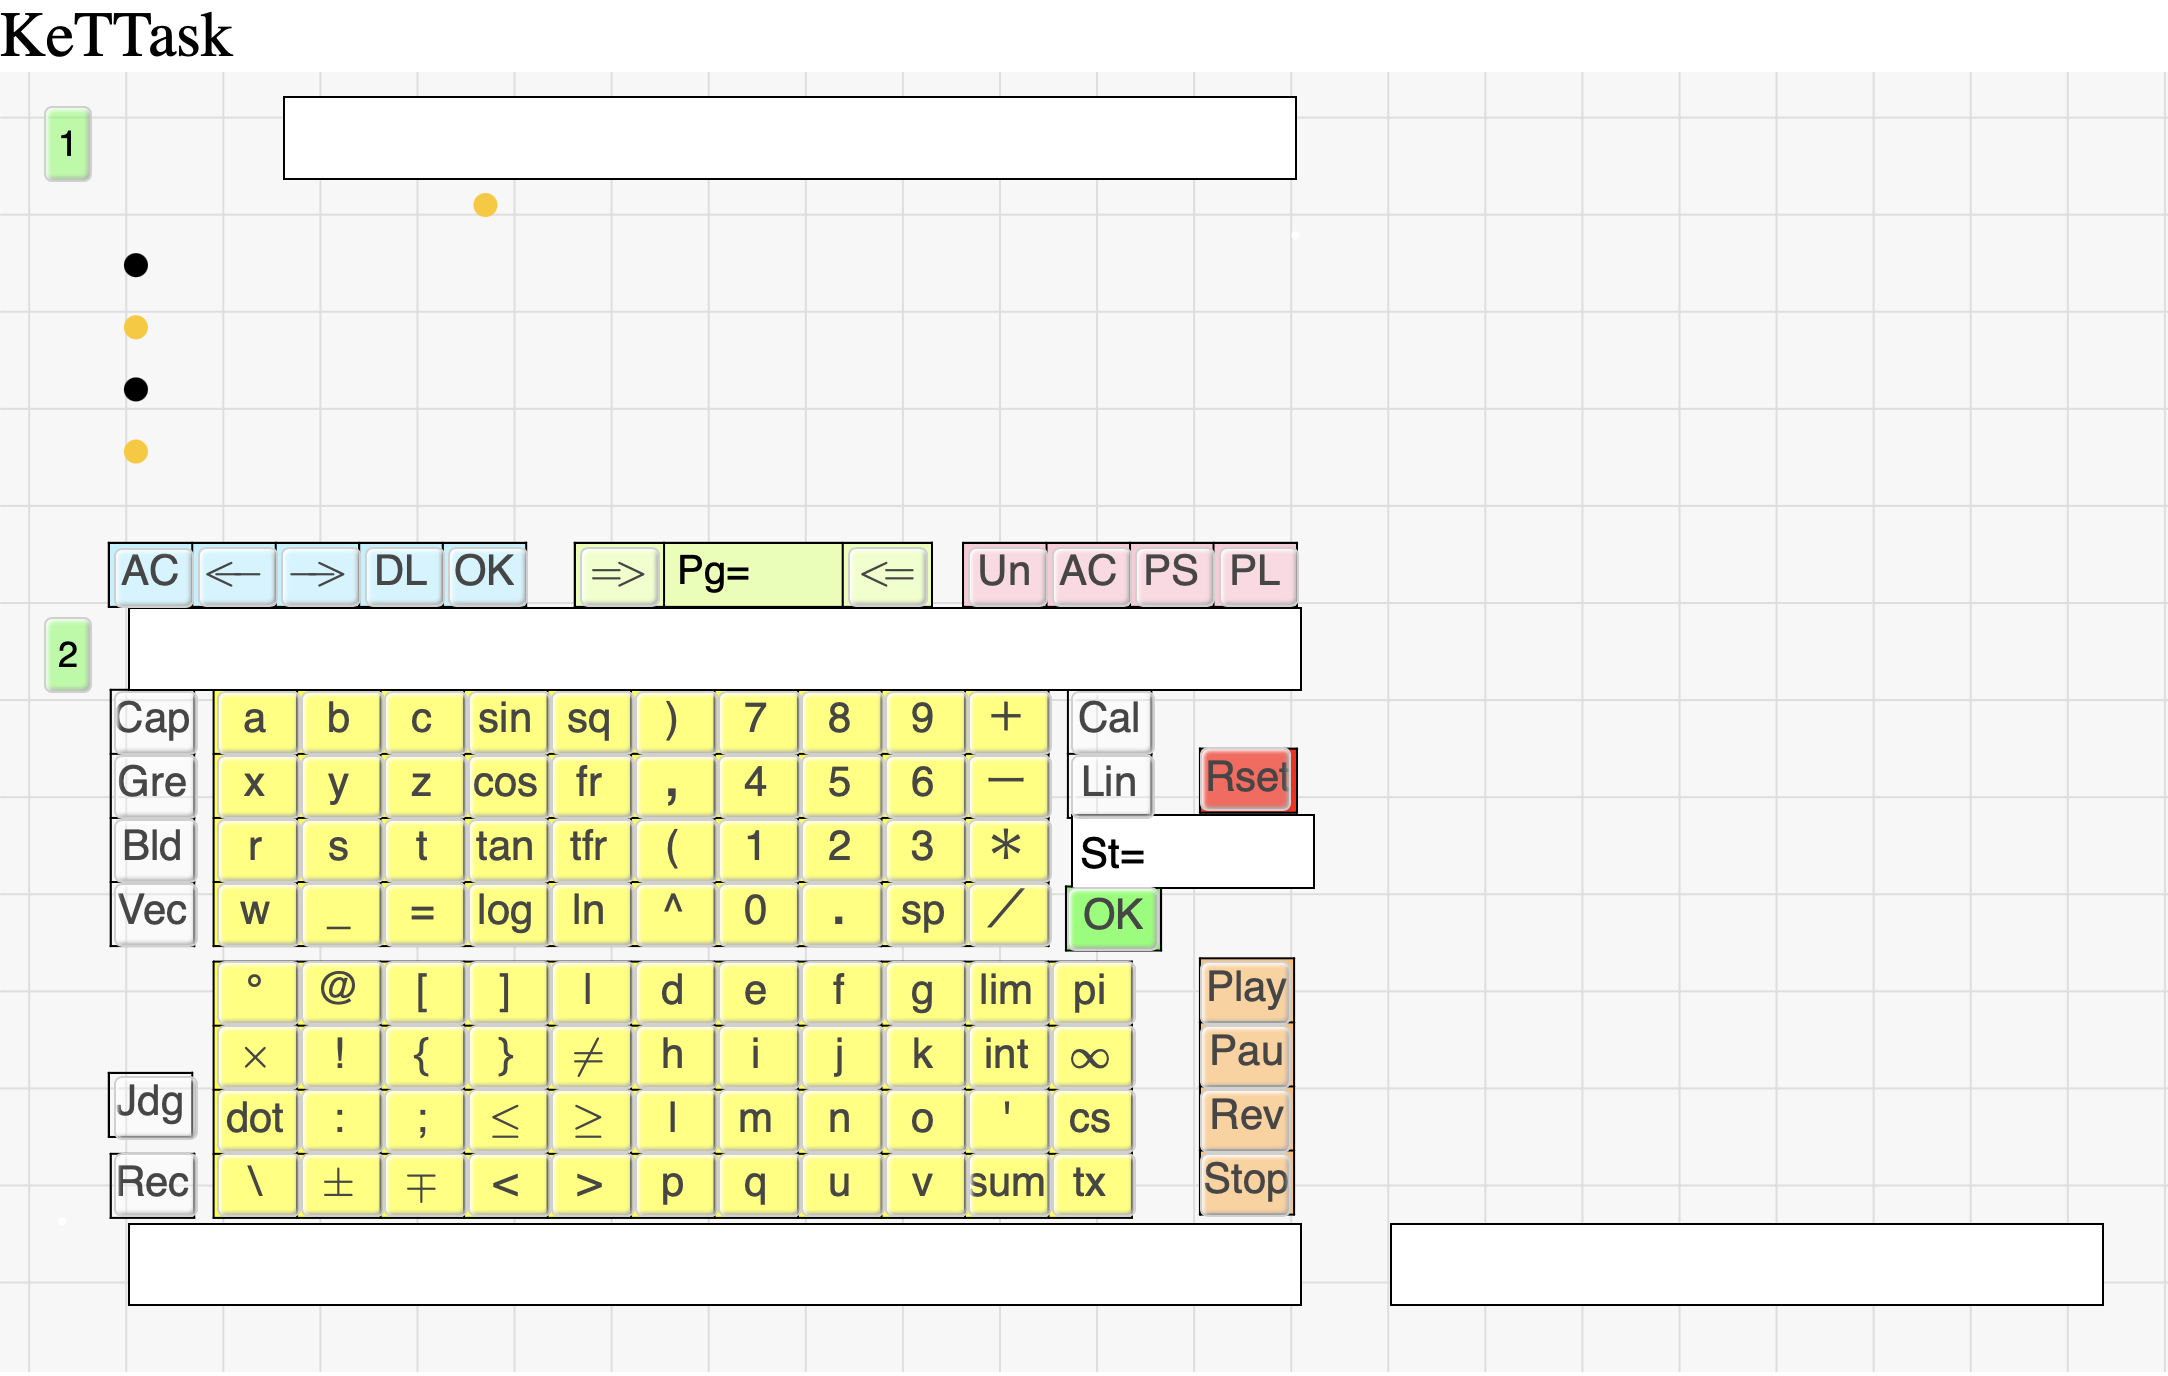
\includegraphics[width=100mm]{fig/kettaskinita.png}
}
\end{layer}

%%%%%%%%%%%%

%%%%%%%%%%%%%%%%%%%%


\sameslide

\vspace*{18mm}

\slidepage
\enminit
\textinit[115]

\begin{layer}{120}{0}
\putnotes{65}{4}{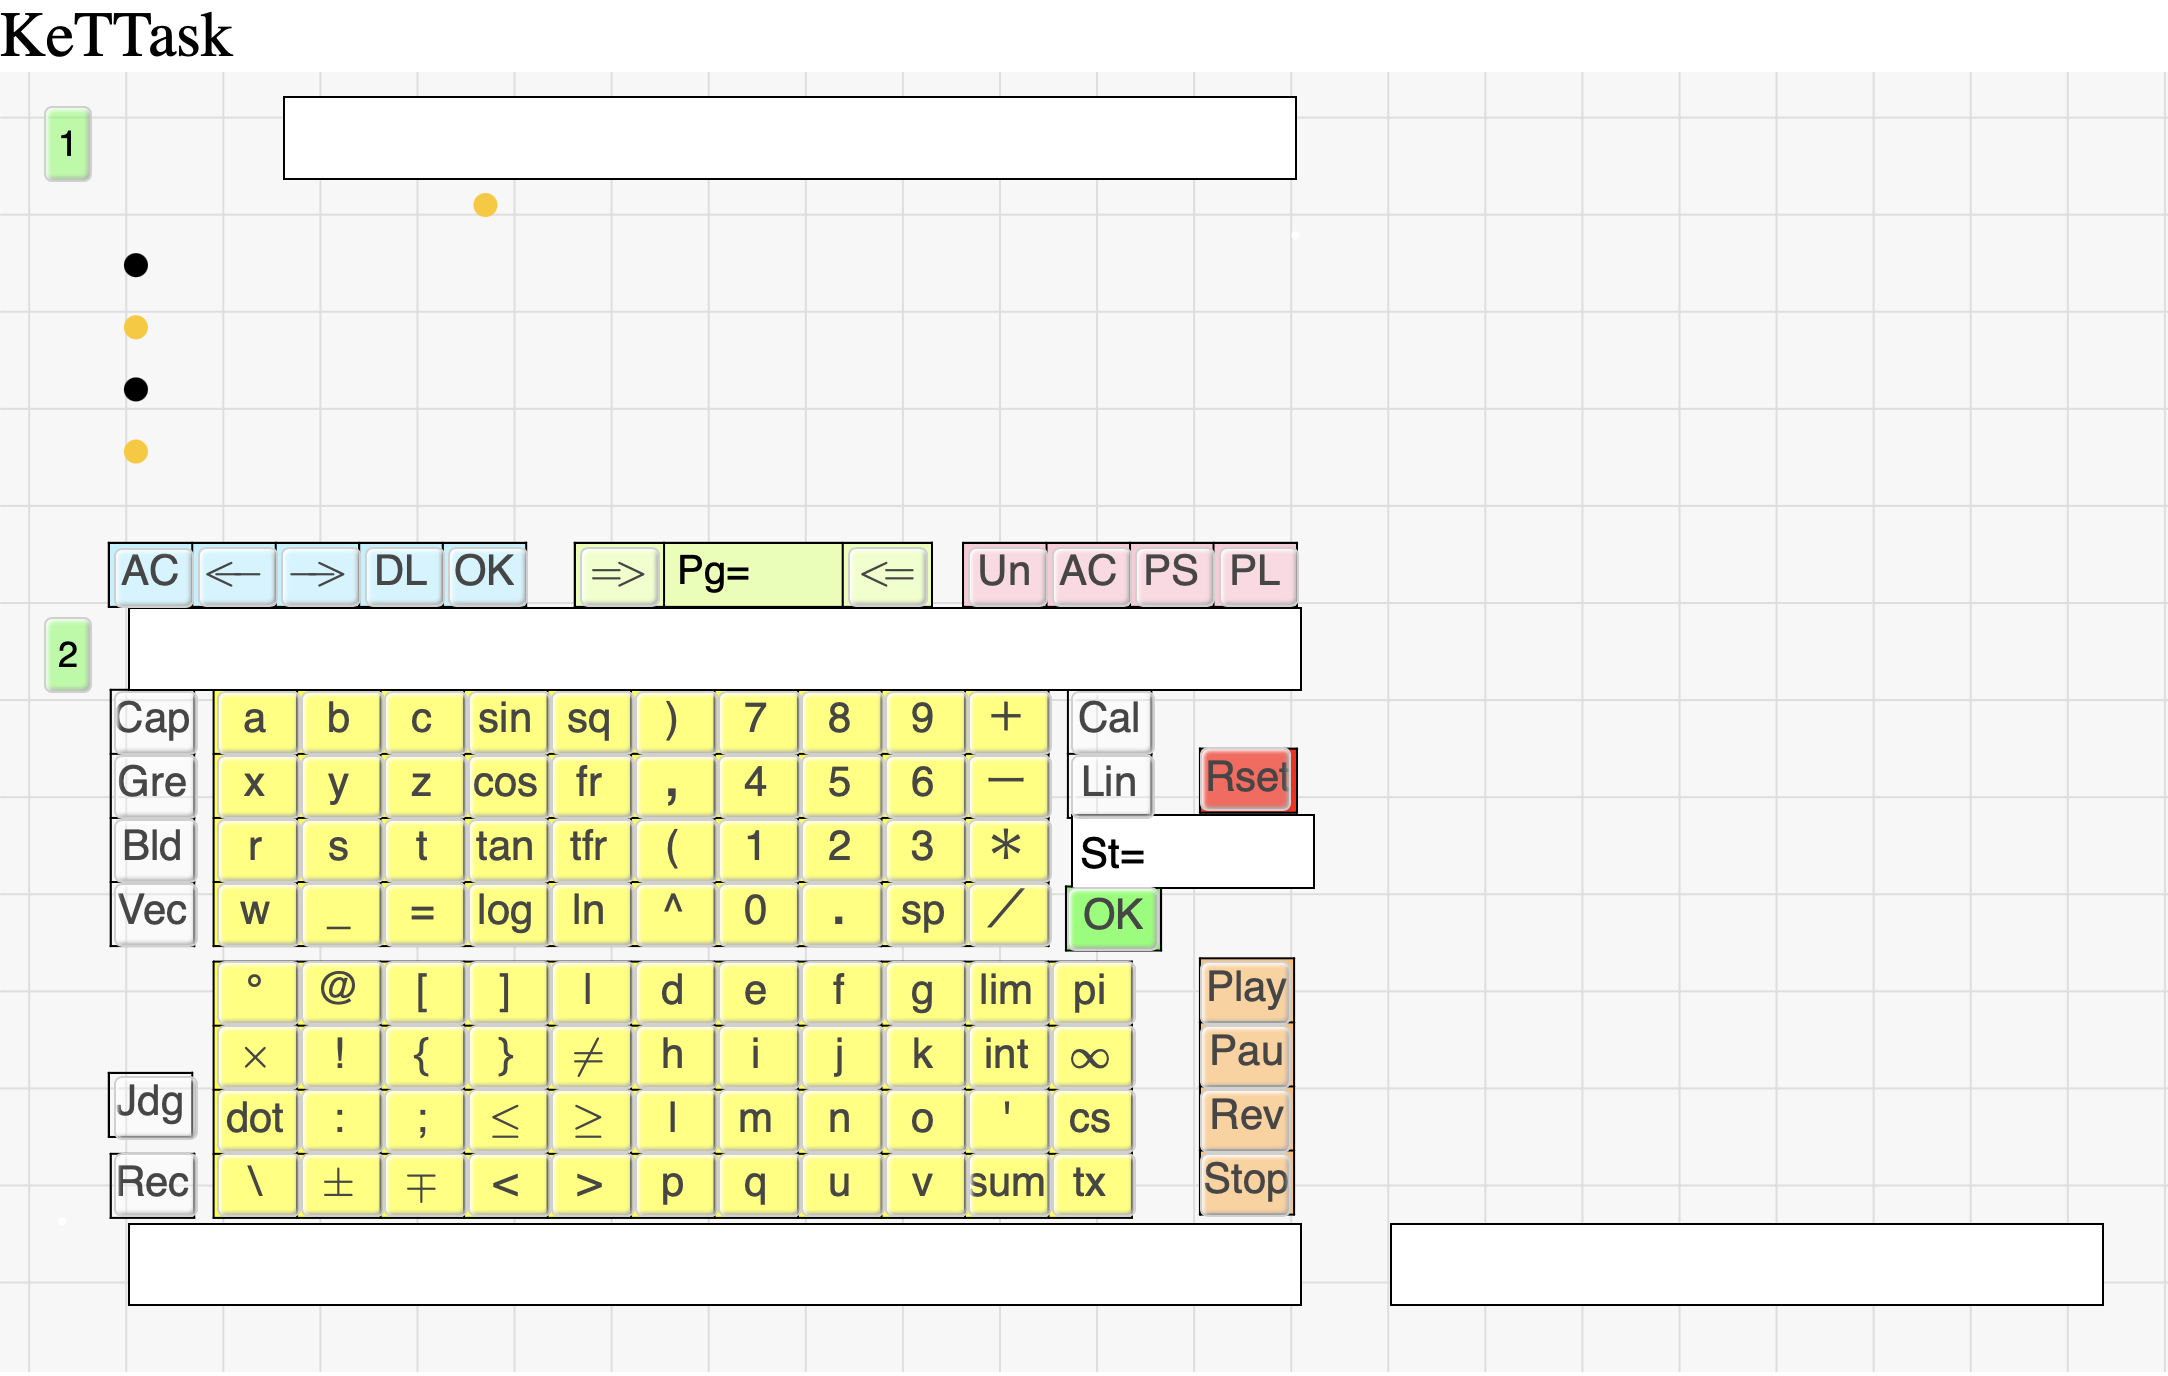
\includegraphics[width=100mm]{fig/kettaskinita.png}
}
\addtext[62]{8}{}{\normalsize This is algebrite boundle version. (There is the Jdg button)}
\end{layer}


\newslide{How to create kettask(xxx)a.html}

\vspace*{18mm}

\slidepage
\enminit
\textinit[100]

\begin{layer}{120}{0}
\addtext[-4]{8}{\ten}{Launch `toolketmathE.cdy'}
%%\textinit[45]
\addtext[-2]{8}{\ten}{Click `1.taskline' and 'Go'}
%%\putnotesw{123}{10}{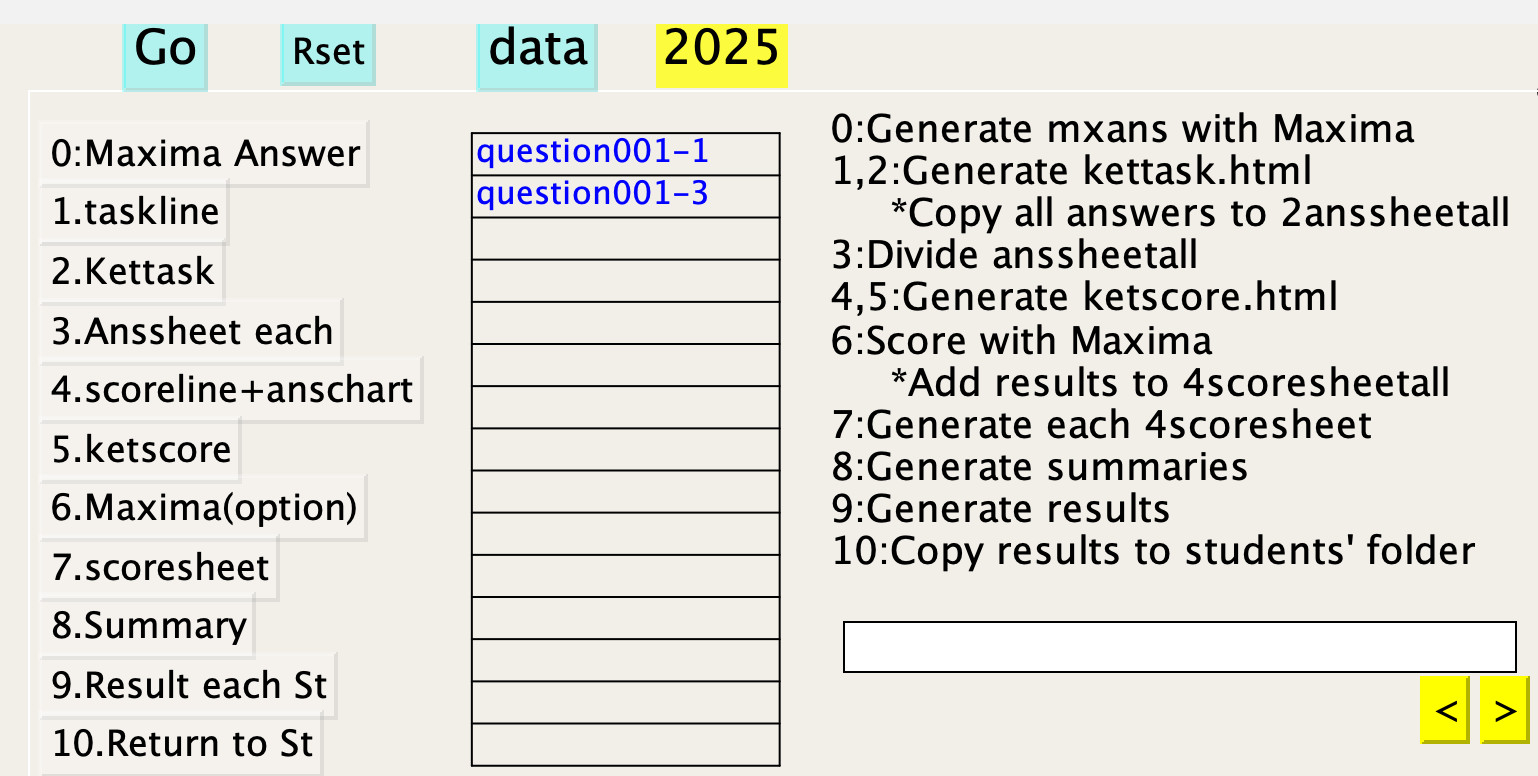
\includegraphics[width=60mm]{fig/toolketmath1a.png}}
\end{layer}

%%%%%%%%%%%%

%%%%%%%%%%%%%%%%%%%%


\sameslide

\vspace*{18mm}

\slidepage
\enminit
\textinit[100]

\begin{layer}{120}{0}
\addtext[-4]{8}{\ten}{Launch `toolketmathE.cdy'}
\addtext[-2]{8}{\ten}{Click `1.taskline' and 'Go'}
\addtext[-2]{8}{\ten}{Click `2.Ketask', select file}\\
\addtext[-2]{50}{}{kettaskorgvEa and `Go'}
\putnotes{63}{30}{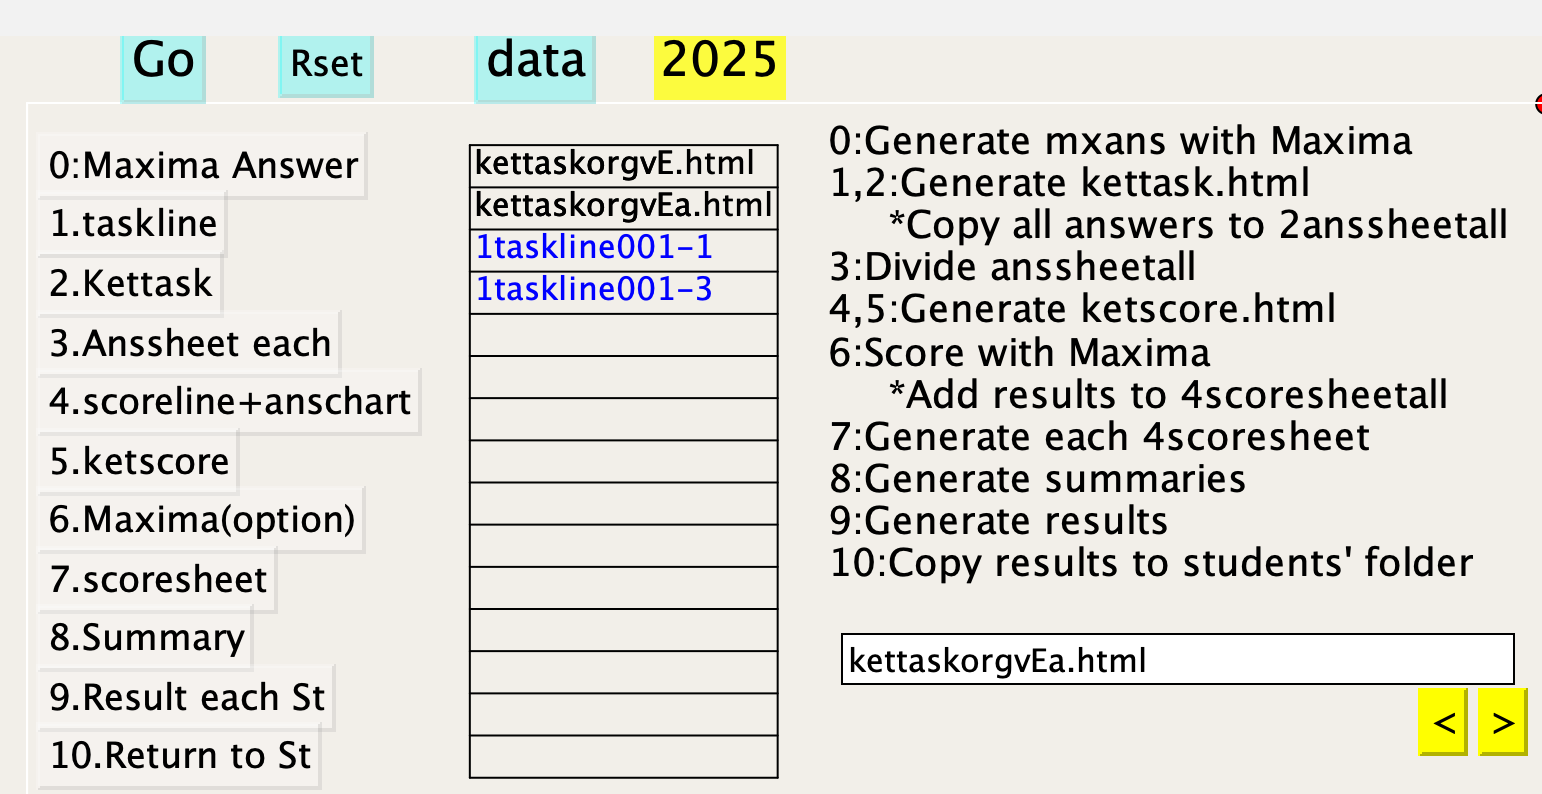
\includegraphics[width=95mm]{fig/toolketmath2a.png}}
\end{layer}


\newslide{How to use kettaska.html}

\vspace*{18mm}

\slidepage
\enminit
\textinit
\vspace{2mm}

{\normalsize

\begin{layer}{120}{0}
\putnotese{3}{2}{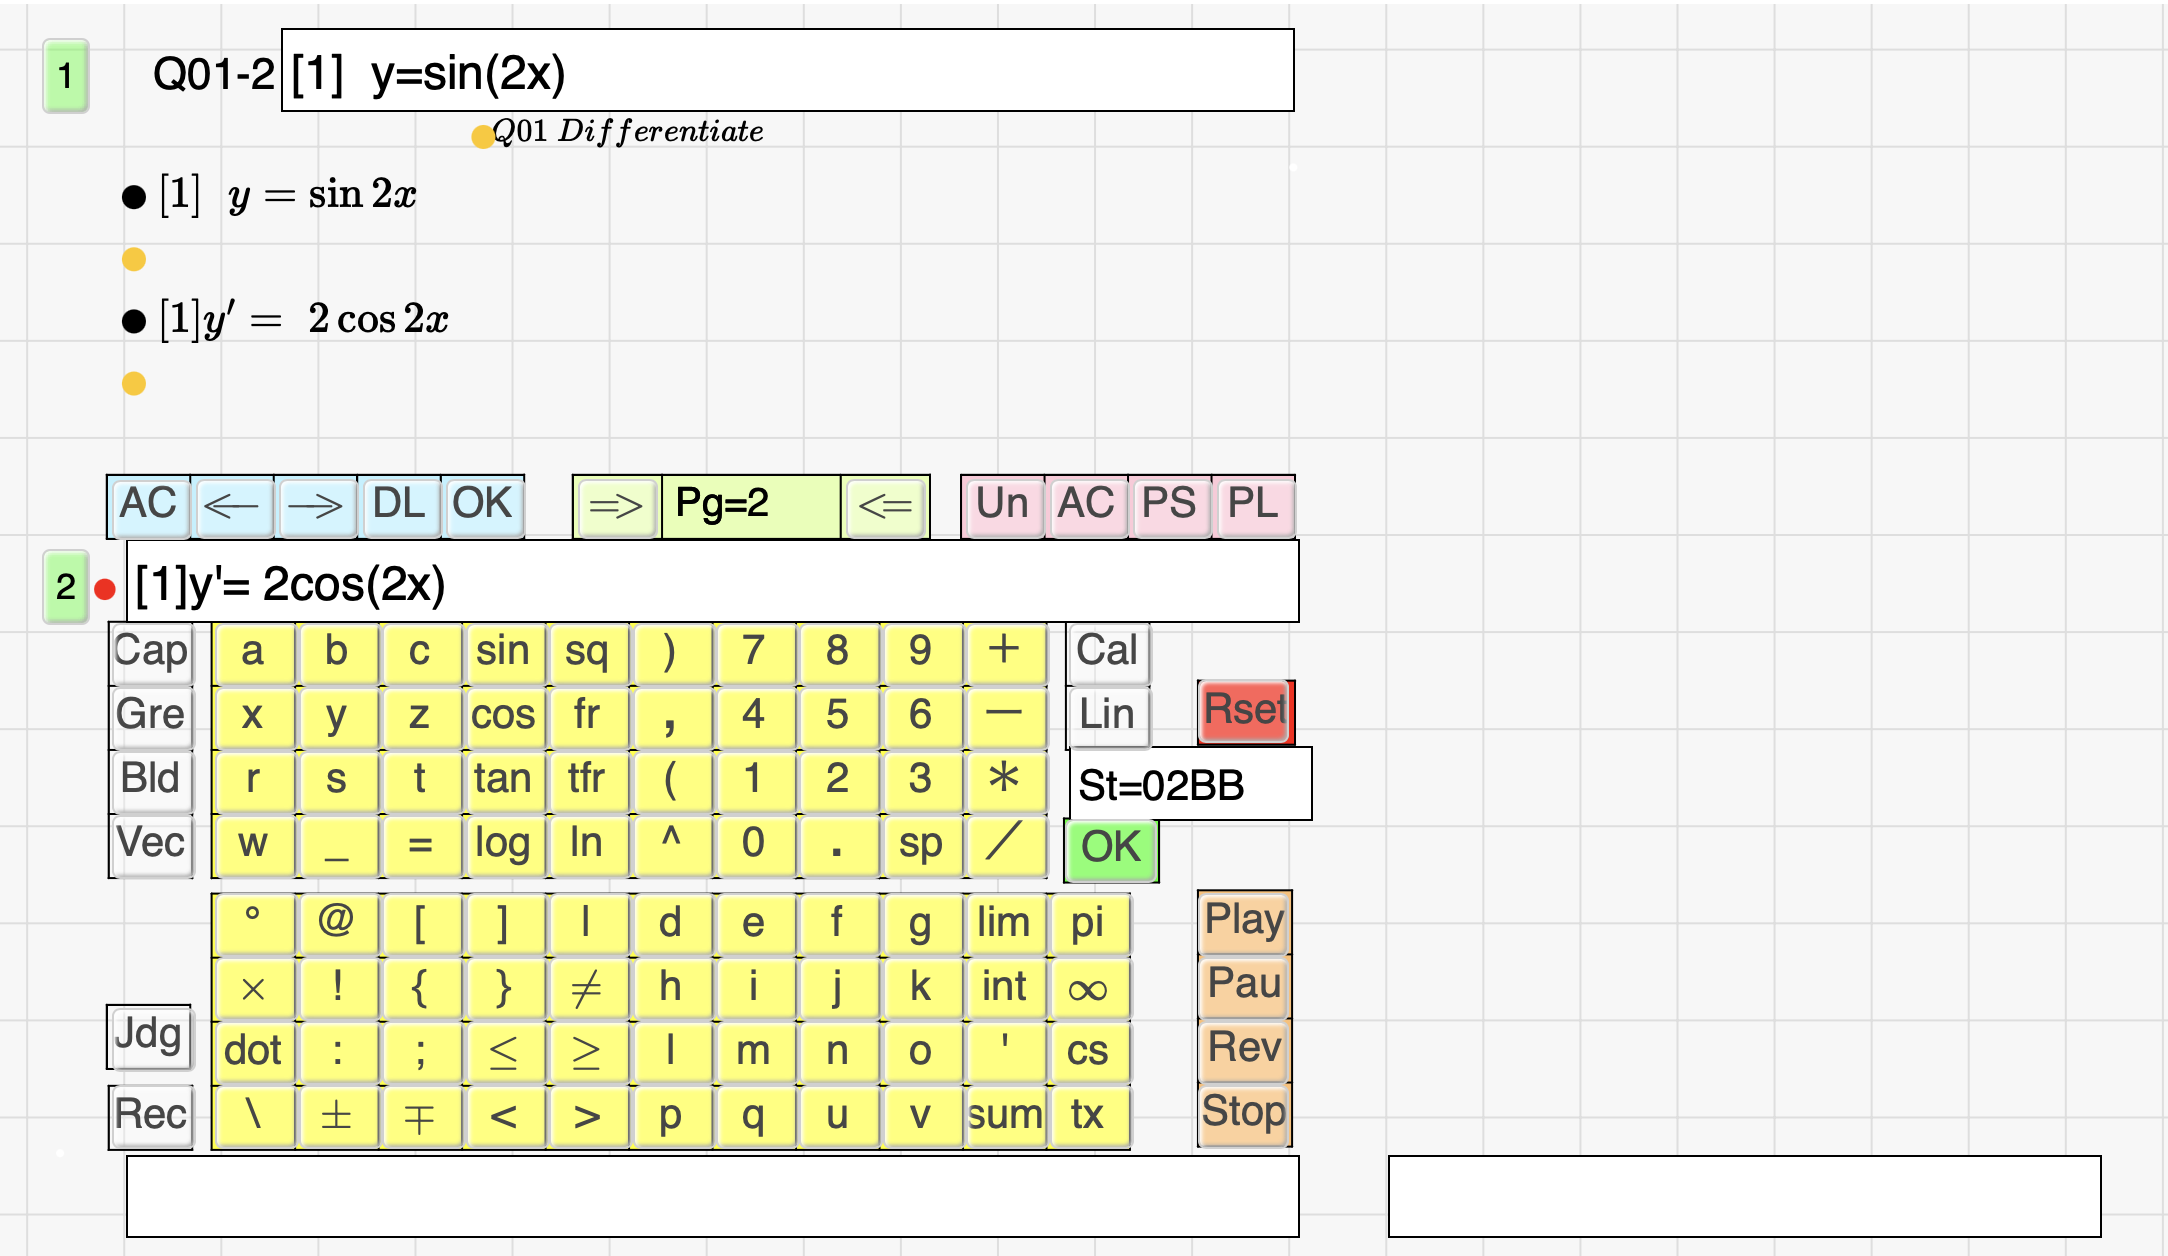
\includegraphics[width=120mm]{fig/kettaska10.png}}
\addtext[-8]{78}{\pnp}{Initial Screen}\adde
\addtext[-4]{78}{\pnp}{St=num, Click \scalebox{.9}{\fcolorbox{black}{green}{\sf OK}}}\adde
\addtext[-2]{78}{\pnp}{Confirm StudentID}\adde
\addtext[-4]{78}{\pnp}{Click \scalebox{.9}{\fcolorbox{black}{green}{\sf OK}} again}\adde
\addtext[-3]{78}{\pnp}{Click \scalebox{.9}{\fcolorbox{black}{mygreen}{\sf $=\!>\!$}}}\adde
\addtext[-3]{78}{\pnp}{Input \fcolorbox{black}{yellow}{\sf 2}}\adde
\addtext[-3]{78}{\pnp}{Click \fcolorbox{black}{yellow}{\sf cos}}\adde
\addtext[-3]{78}{\pnp}{Input 2x}\adde
\addtext[-4]{78}{\pnp}{Click \scalebox{.9}{\fcolorbox{black}{cyan!20}{\sf$-\!\!\!>\!$}}('?' moves)}\adde
\addtext[-3]{78}{\pnp}{Click \scalebox{.9}{\fcolorbox{black}{cyan!20}{\sf OK}}}\adde
\addtext[-3]{82}{}{'?' disappears}
\end{layer}

}
%%%%%%%%%%%%

%%%%%%%%%%%%%%%%%%%%


\sameslide

\vspace*{18mm}

\slidepage
\enminit
\textinit
\vspace{2mm}

{\normalsize

\begin{layer}{120}{0}
\putnotese{3}{2}{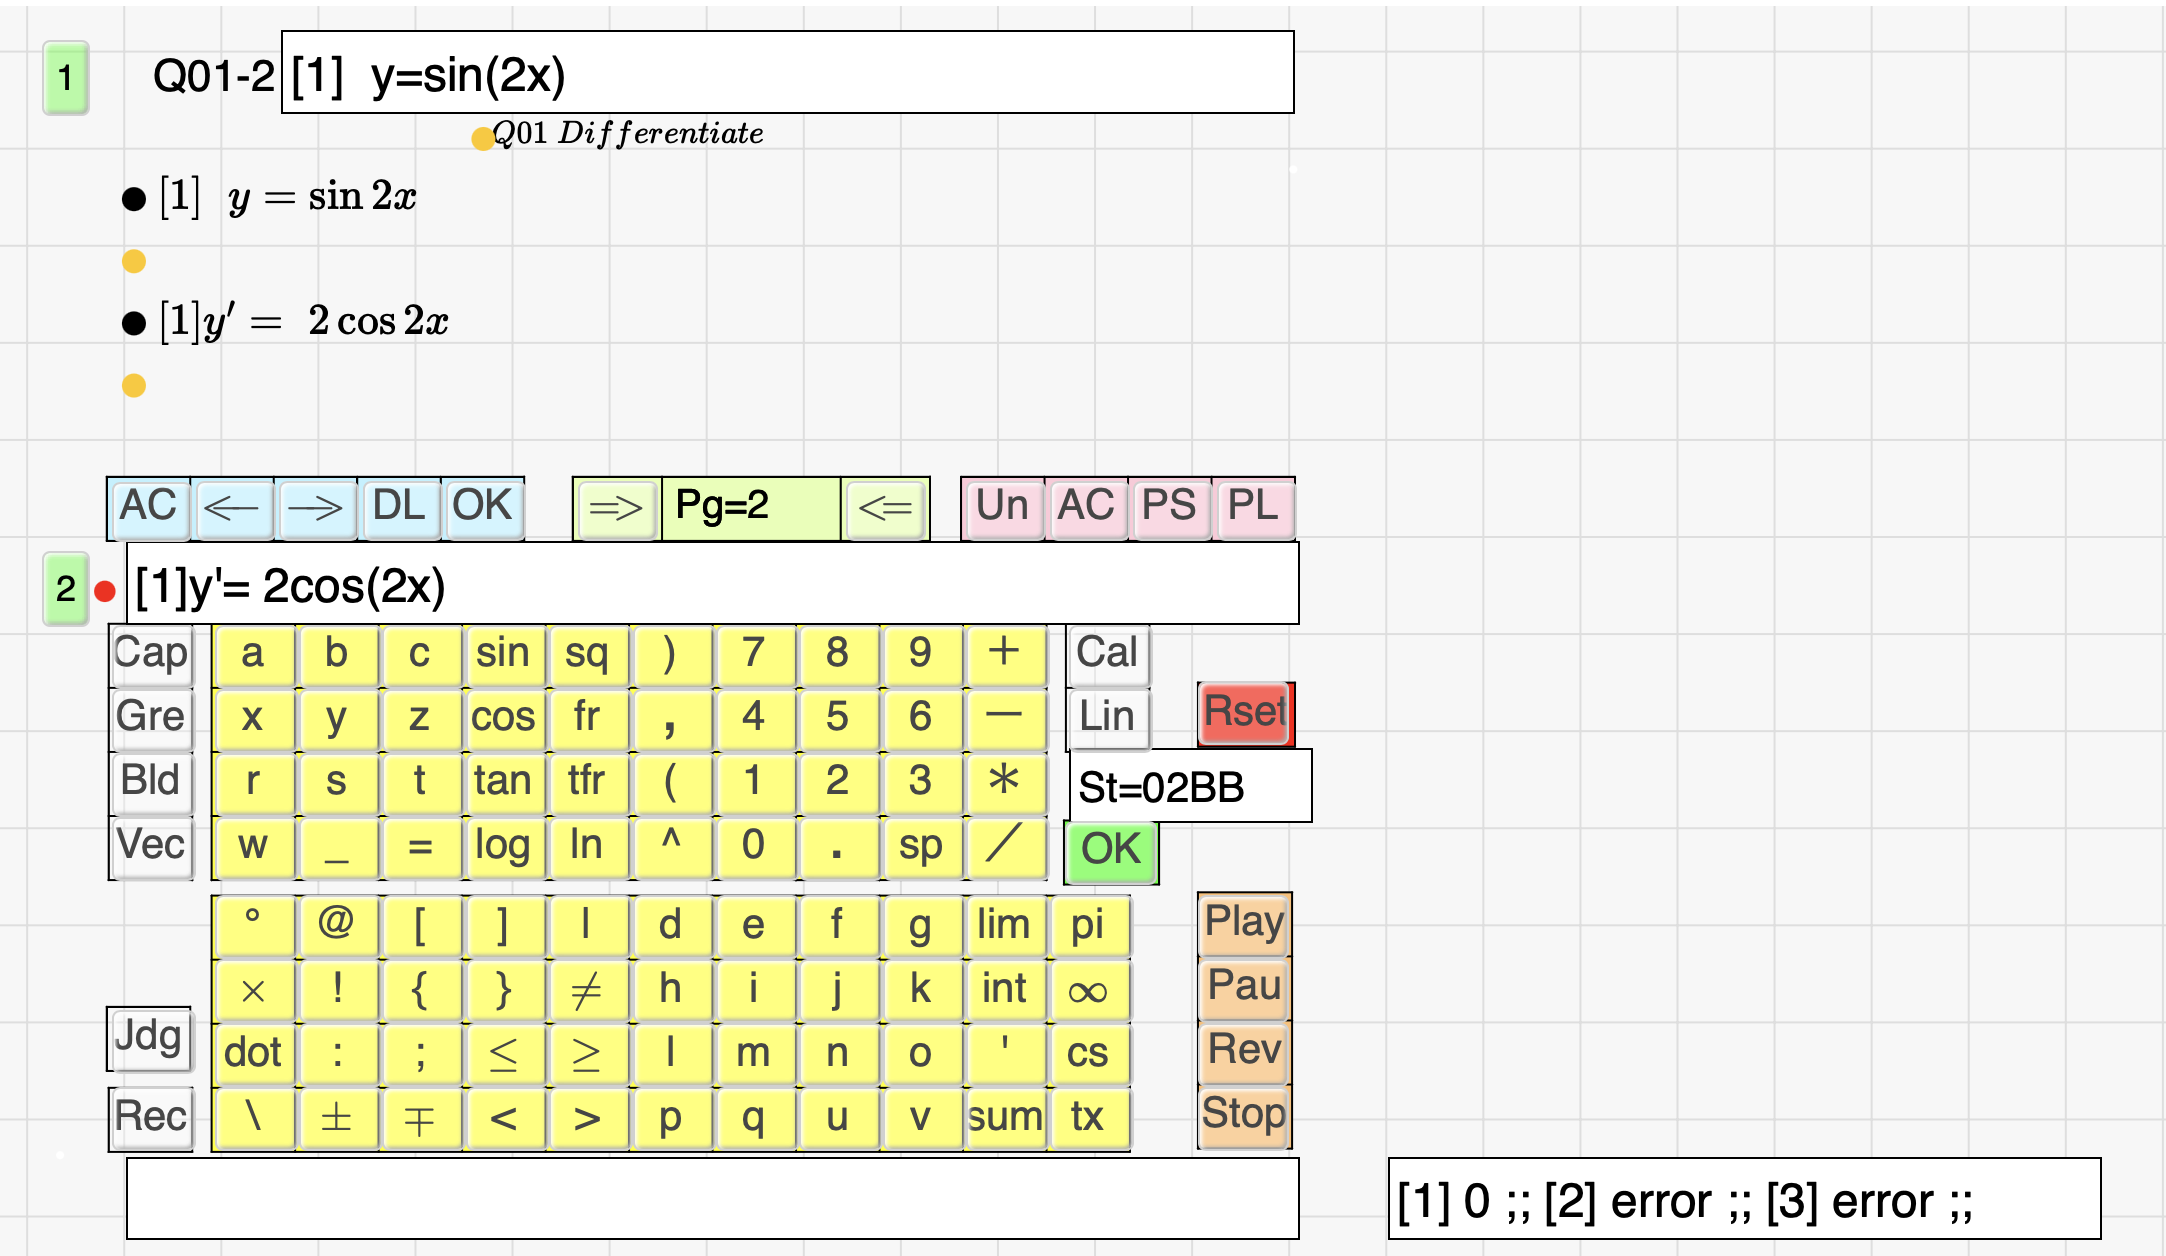
\includegraphics[width=120mm]{fig/kettaska11.png}}
\addtext[-8]{78}{\pnp}{Initial Screen}\adde
\addtext[-4]{78}{\pnp}{St=num, Click \scalebox{.9}{\fcolorbox{black}{green}{\sf OK}}}\adde
\addtext[-2]{78}{\pnp}{Confirm StudentID}\adde
\addtext[-4]{78}{\pnp}{Click \scalebox{.9}{\fcolorbox{black}{green}{\sf OK}} again}\adde
\addtext[-3]{78}{\pnp}{Click \scalebox{.9}{\fcolorbox{black}{mygreen}{\sf $=\!>\!$}}}\adde
\addtext[-3]{78}{\pnp}{Input \fcolorbox{black}{yellow}{\sf 2}}\adde
\addtext[-3]{78}{\pnp}{Click \fcolorbox{black}{yellow}{\sf cos}}\adde
\addtext[-3]{78}{\pnp}{Input 2x}\adde
\addtext[-4]{78}{\pnp}{Click \scalebox{.9}{\fcolorbox{black}{cyan!20}{\sf$-\!\!\!>\!$}}('?' moves)}\adde
\addtext[-3]{78}{\pnp}{Click \scalebox{.9}{\fcolorbox{black}{cyan!20}{\sf OK}}}\adde
\addtext[-3]{82}{}{'?' disappears}
\addtext[-4]{78}{\pnp}{Click \scalebox{.85}{\fbox{\sf Jdg}}}\adde
\end{layer}

}

\sameslide

\vspace*{18mm}

\slidepage
\enminit
\textinit
\vspace{2mm}

{\normalsize

\begin{layer}{120}{0}
\putnotese{3}{2}{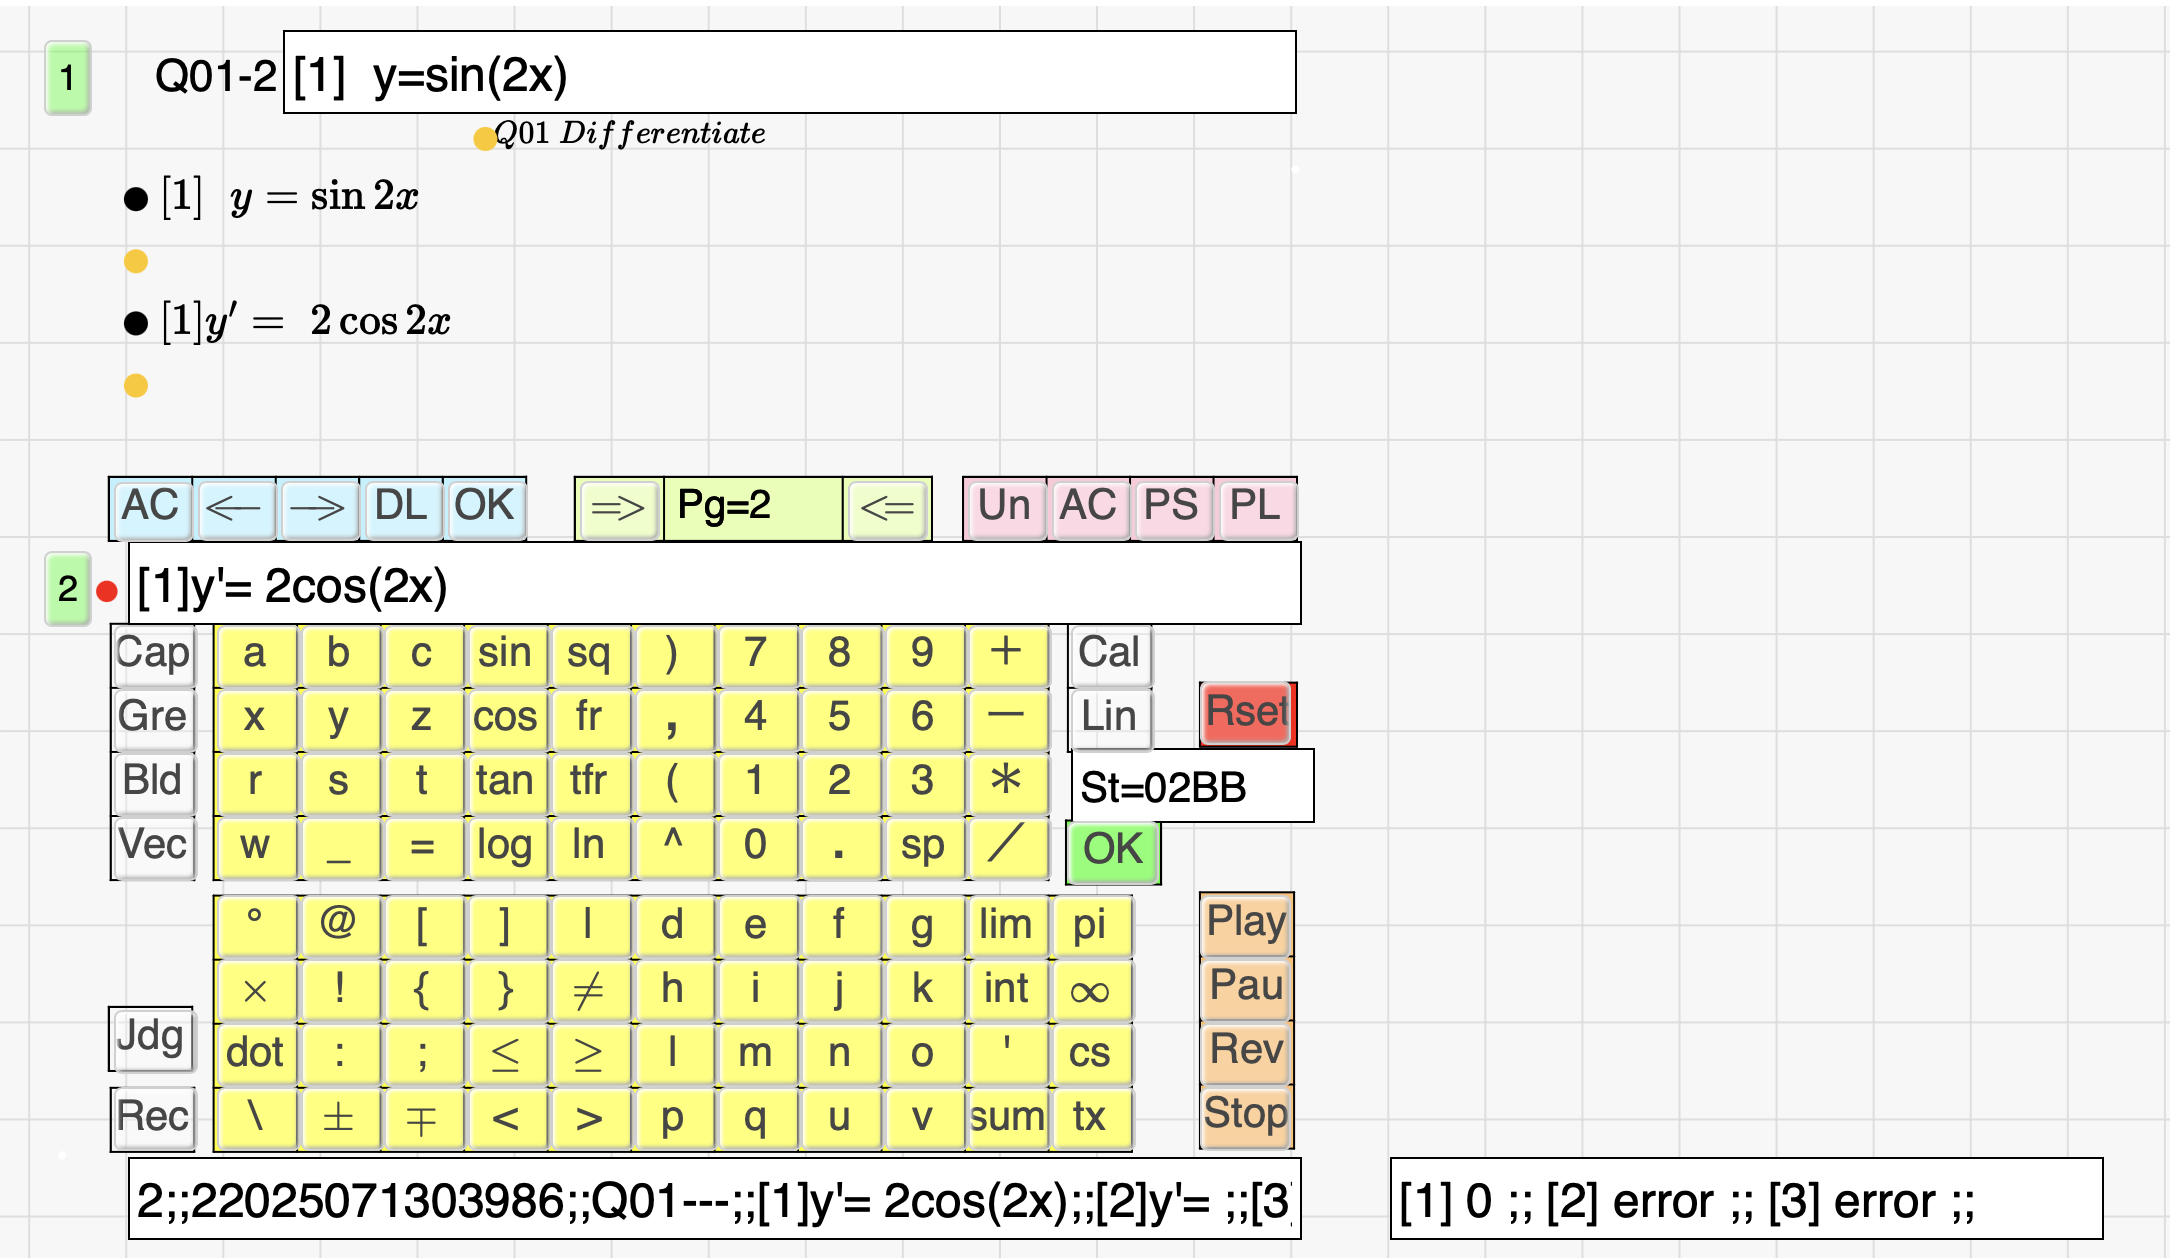
\includegraphics[width=120mm]{fig/kettaska12.png}}
\addtext[-8]{78}{\pnp}{Initial Screen}\adde
\addtext[-4]{78}{\pnp}{St=num, Click \scalebox{.9}{\fcolorbox{black}{green}{\sf OK}}}\adde
\addtext[-2]{78}{\pnp}{Confirm StudentID}\adde
\addtext[-4]{78}{\pnp}{Click \scalebox{.9}{\fcolorbox{black}{green}{\sf OK}} again}\adde
\addtext[-3]{78}{\pnp}{Click \scalebox{.9}{\fcolorbox{black}{mygreen}{\sf $=\!>\!$}}}\adde
\addtext[-3]{78}{\pnp}{Input \fcolorbox{black}{yellow}{\sf 2}}\adde
\addtext[-3]{78}{\pnp}{Click \fcolorbox{black}{yellow}{\sf cos}}\adde
\addtext[-3]{78}{\pnp}{Input 2x}\adde
\addtext[-4]{78}{\pnp}{Click \scalebox{.9}{\fcolorbox{black}{cyan!20}{\sf$-\!\!\!>\!$}}('?' moves)}\adde
\addtext[-3]{78}{\pnp}{Click \scalebox{.9}{\fcolorbox{black}{cyan!20}{\sf OK}}}\adde
\addtext[-3]{82}{}{'?' disappears}
\addtext[-4]{78}{\pnp}{Click \scalebox{.85}{\fbox{\sf Jdg}}}\adde
\addtext[-3]{78}{\pnp}{Click \scalebox{.85}{\fbox{\sf Rec}}}
\end{layer}

}

\newslide{How to use Algebrite}

\vspace*{18mm}

\slidepage
\enminit
\textinit[110]

\begin{layer}{120}{0}
{\large
\addtext{8}{\ten}{We can use the command `{\tt\color{red}exealg}' in {\tt kettaska.html}.}
\addtext[-2]{10}{}{Example:}
\addtext[-2]{16}{}{{\tt tmqu1="fr(1,2)x\textasciicircum(2)";//} formulas in KetMath rule}
\addtext[-2]{16}{}{\tt tmqu2=Tomaxform(tmqu1);}
\addtext[-2]{16}{}{{\tt // Tomaxform} change formulas for algebrite}
\addtext[-2]{16}{}{\tt tmqu3="d("+tmqu2+",x)";}
\addtext[-2]{16}{}{{\tt // d(f,x)} is a function of algebrite}
\addtext[-2]{16}{}{\tt out1 = exealg(tmqu3);}
\addtext{12}{}{then out1 is {\tt x\textasciicircum2} that the defferential of tmqu2.}
}
\end{layer}

%%%%%%%%%%%%

%%%%%%%%%%%%%%%%%%%%


\newslide{Judge with Algebrite}

\vspace*{18mm}

\slidepage
\enminit
\textinit[110]

\begin{layer}{120}{0}
{\large
\addtext[-4]{8}{\ten}{We use the command `{\tt\color{red}exealg}' to judge with Algebrite.}
\addtext{10}{}{Example:}
\addtext[-2]{16}{}{\tt tans3=Tomaxform(tans2);}
\addtext[-2]{16}{}{\tt tmqu3="d("+tmqu2+",x)";}
\addtext[-2]{16}{}{\tt jdgfun=tmqu3+"-("+tans3+")";}
\addtext[-2]{16}{}{\tt jdgout = exealg(jdgfun);}
\addtext{8}{\ten}{{\tt tans2} is the student's answer.}
\addtext[-2]{8}{\ten}{Instead of inputting the correct answer {\tt tmqu3} directly, we let Algebrite compute it.}
\addtext[3]{8}{\ten}{`{\tt 3x\textasciicircum(2)-12}' and `{\tt 3(x\textasciicircum(2)-4)}' are mathematically equivalent and correct according to Algebrite.}
}
\end{layer}

%%%%%%%%%%%%

%%%%%%%%%%%%%%%%%%%%


\newslide{How to embed Script to Judge}

\vspace*{18mm}

\slidepage
\enminit
\textinit[113]

\begin{layer}{120}{0}
\addtext[-4]{6}{}{Embed it the same way you would embed a drawn graph.}
\end{layer}

%%%%%%%%%%%%

%%%%%%%%%%%%%%%%%%%%


\sameslide

\vspace*{18mm}

\slidepage
\enminit
\textinit[113]

\begin{layer}{120}{0}
\putnotesw{125}{12}{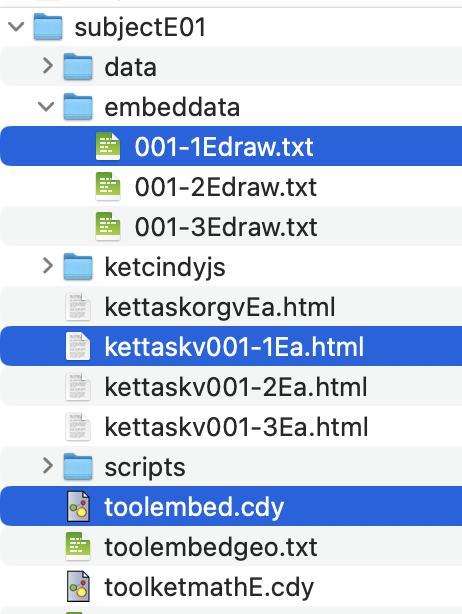
\includegraphics[width=40mm]{fig/HowtoEmbedScript.png}}
\addtext[-4]{6}{}{Embed it the same way you would embed a drawn graph.}
\addtext[6]{6}{\pnp}{Create a KeTTask file }\\
\addtext[-2]{15}{}{\normalsize(\mbox{kettask001-01Ea}.html for example)}\adde
\addtext[-2]{6}{\pnp}{Create `01-1draw.txt' in }\\
\addtext[-2]{14}{}{the folder `embeddata'.}\adde
\addtext{6}{\pnp}{Change the name of the }\\
\addtext[-2]{15}{}{second button from \fcolorbox{black}{cyan!70}{\sf Start} }\\
\addtext[-2]{15}{}{to \fcolorbox{black}{cyan!70}{\sf Embed}.}\adde
\addtext{6}{\pnp}{Push \fcolorbox{black}{cyan!70}{\sf OK} $\Rightarrow$ \fcolorbox{black}{cyan!70}{\sf Embed}.}
\addtext[2]{6}{\ten}{{\color{blue}I will explain with a sample file.}}
\end{layer}


\newslide{Conclusion}

\vspace*{18mm}

\slidepage
\enminit
\textinit[100]

\begin{layer}{120}{0}
\addtext[-3]{8}{\pnp}{Students can judge their answers semantically using algebrite.}\adde
\addtext[10]{8}{\pnp}{Improving a judge script with coraboration of Algebrite and KeTCindy Script is Future work.}\adde
\addtext[16]{8}{\pnp}{Another future work is to investigate whether semantic self-assessment via the [Jdg] button is educationally effective.}\adde
\end{layer}

%%%%%%%%%%%%

%%%%%%%%%%%%%%%%%%%%


\newslide{}

\vspace*{18mm}

\slidepage

\begin{layer}{120}{0}
\textinit[120]
\putnotes{62}{25}{\scalebox{0.9}{\Huge Thank you for your attention}}
\end{layer}


\sameslide

\vspace*{18mm}

\slidepage

\begin{layer}{120}{0}
\textinit[120]
\putnotes{62}{25}{\scalebox{0.9}{\Huge Thank you for your attention}}
\putnotes{62}{40}{
\includegraphics[width=80mm]{fig/thankyouGreek.png}}
\putnotes{62}{55}{
\includegraphics[width=80mm]{fig/thankyouJapan.png}}
\end{layer}

\label{pageend}\mbox{}

\end{document}
